\documentclass[EJP,preprint]{ejpecp}
% A local Lamperti law for the occupation count with infinite-mean runs.
% The class ejpecp is in TeX Live. Build: pdflatex problem131_lamperti.tex, three times.
% Disclosure statement: the author decides whether one is needed and what it says.

\usepackage{booktabs}
\usepackage[shortlabels]{enumitem}

% ---------- theorem environments (the class provides theorem, lemma,
% proposition, corollary, definition, example, remark, conjecture and its other
% theorem-like environments, numbered within sections; the lettered main
% theorems are added here) ----------
\theoremstyle{ejpecpbodyit}
\newtheorem{introtheorem}{Theorem}
\renewcommand{\theintrotheorem}{\Alph{introtheorem}}

% ---------- notation macros ----------
\newcommand{\Z}{\mathbb{Z}}
\newcommand{\N}{\mathbb{N}}
\newcommand{\R}{\mathbb{R}}
\newcommand{\C}{\mathbb{C}}
\newcommand{\E}{\mathbb{E}}
\newcommand{\Prob}{\mathbb{P}}
\newcommand{\ones}{\mathbf{1}}
\newcommand{\plus}{{+}}
\newcommand{\minus}{{-}}
\newcommand{\sgn}{\sigma}
\newcommand{\osgn}{\bar\sigma}
\newcommand{\La}{L_{\alpha,b}}
\newcommand{\Gam}{\Gamma_{\!\alpha}}

\graphicspath{{figures/}}
\emergencystretch=1em

\TITLE{A local Lamperti law for the occupation count of a lattice L\'evy walk with infinite-mean runs}
\SHORTTITLE{A local Lamperti law}
\AUTHORS{Arjun Pemmasani\footnote{Department of Mathematics, Harvey Mudd College,
Claremont, CA 91711, USA. \BEMAIL{apemmasani@hmc.edu}}}
\KEYWORDS{Lamperti law; generalized arcsine law; occupation time; alternating renewal
process; local limit theorem; strong renewal theorem; L\'evy walk; infinite mean}
\AMSSUBJ{60K05; 60F05; 60G50}
\AMSSUBJSECONDARY{60G52; 60K15; 82C41}
\SUBMITTED{}
\ACCEPTED{}
\ABSTRACT{A lattice L\'evy walk moves in runs of alternating direction whose
independent lengths have regularly varying tails of index $\alpha\in(0,1)$. Let
$A_N$ be the number of right steps among the first $N$. Lamperti's theorem gives
the limit law of $A_N/N$. We prove its local form. The rescaled point
probabilities $N\Prob(A_N=k)$ converge to Lamperti's density at one interior
point if and only if they converge uniformly on compact sets, and this happens if
and only if both run laws satisfy the strong renewal theorem. By the
characterization of Caravenna and Doney, the local law therefore holds with no
further condition when $\alpha>1/2$, and for $\alpha\le1/2$ it holds exactly
under their condition for each run law. We identify the limit directly from the
renewal structure. For equal tails the density is U-shaped if
$\cos(\pi\alpha/2)\ge\alpha$ and W-shaped otherwise, with exactly $1$ or $3$
critical points, which gives the threshold $\alpha=0.5946\ldots$ in closed form.
Near the ends the law is the tail of a run times a renewal mass function, and
under Doney's local condition this boundary layer matches the bulk uniformly, so
the global mode sits at bounded distance from an end for every $\alpha$. For an
arbitrary initial run we give the exact defect in the bulk, a necessary condition,
a sufficient condition, and an exact criterion. An initial run that is finite
almost surely can change the local law in the bulk. We also give a lower bound on
the number of local extrema of the law.}

\begin{document}

\section{Introduction}\label{sec:intro}

A lattice L\'evy walk moves on $\Z$ in runs of alternating direction. The run
lengths are independent, the right runs have one law and the left runs another,
and we assume that both tails are regularly varying with the same index
$\alpha\in(0,1)$. So the runs have infinite mean. Let $A_N$ be the number of right
steps among the first $N$, and put $P_N(k)=\Prob(A_N=k)$ for $0\le k\le N$. The
walk is at $2A_N-N$ after $N$ steps, so $P_N$ is the law of the walk on its natural
lattice, and it is also the law of the occupation count of a discrete-time
alternating renewal process. In the infinite-mean regime $A_N/N$ does not
concentrate. Its limit law is a generalized arcsine law, with density
\begin{equation}\label{eq:lamperti-intro}
 \La(x)=\frac{\sin\pi\alpha}{\pi}\,
 \frac{b\,x^{\alpha-1}(1-x)^{\alpha-1}}{b^2x^{2\alpha}+2b\cos(\pi\alpha)\,x^\alpha(1-x)^\alpha+(1-x)^{2\alpha}},
 \qquad 0<x<1,
\end{equation}
where $b$ is the limit ratio of the left tail to the right tail. This density goes
back to Lamperti~\cite{lamperti1958}, and in the physics literature it is called
the Lamperti distribution~\cite{margolinbarkai2006,zdk2015}. This paper is about
the local form of this law, at single points $k$.

\subsection{The local Lamperti law}\label{sec:intro-local}

Write $T_\pm(n)=\Prob(X_\pm\ge n)$ for the tails of the two run lengths. A renewal
law with a tail $T$ of index $\alpha\in(0,1)$ satisfies the strong renewal theorem
(SRT) if its renewal mass function $u$ satisfies
\[
 u(n)\sim\frac{\sin\pi\alpha}{\pi}\,\frac1{nT(n)}\qquad(n\to\infty).
\]
For $\alpha>1/2$ this always holds under aperiodicity, by Garsia and
Lamperti~\cite{garsialamperti1963} and Erickson~\cite{erickson1970}. For
$\alpha\le1/2$ it can fail, and Caravenna and Doney~\cite{caravennadoney2019}
found the exact condition. Our first theorem says that the local Lamperti law is
equivalent to the strong renewal theorem for both run laws.

\begin{introtheorem}[the local Lamperti law]\label{thm:local}
Assume that $T_\plus$ and $T_\minus$ are regularly varying with index $-\alpha$,
$0<\alpha<1$, that $T_\minus(n)/T_\plus(n)\to b\in(0,\infty)$, and that the run laws
are aperiodic. Let the walk start with a fresh run of either sign. Then the
following are equivalent.
\begin{enumerate}[(i)]
\item $NP_N(\lfloor x_0N\rfloor)\to\La(x_0)$ for one $x_0\in(0,1)$.
\item $NP_N(k)=\La(k/N)+o(1)$ uniformly over $k$ with $k/N$ in each compact
subset of $(0,1)$.
\item Both run laws satisfy the strong renewal theorem.
\end{enumerate}
\end{introtheorem}

With the theorem of Caravenna and Doney this gives a complete answer. For
$\alpha>1/2$ the local law holds under regular variation and aperiodicity alone.
For $\alpha\le1/2$ it holds if and only if each run law satisfies their condition,
which we recall in Lemma~\ref{lem:cd}, and Doney's local condition
$f_\pm(n)=O(T_\pm(n)/n)$ suffices. A single interior point already forces the
strong renewal theorem for both laws. Without it the lower half of the local law still
holds, $\liminf_N(NP_N(k)-\La(k/N))\ge0$ uniformly on compact sets, and the failure of the
strong renewal theorem shows up as an excess at every interior point
(Corollary~\ref{cor:lower}).

The proof does not need a bivariate local renewal theorem. An exact identity
writes $P_N(k)$ through the convolution powers of the two run laws, sorted by the
number $m$ of completed runs. For $m$ of order $1/T_\plus(N)$ the local limit
theorem of Gnedenko gives a Riemann sum for an explicit double integral. The key
estimate, Lemma~\ref{lem:key}, bounds the probability that the $(m+1)$-th run covers
a level $k$ by $CT(k)$ uniformly in $m$, under regular variation alone. It
decouples the two signs for small $m$, and the contribution of small $m$ of each
sign is then exactly the quantity that Caravenna and Doney show to be
asymptotically negligible if and only if the strong renewal theorem holds. The
limit comes out as a double integral over stable densities, and we identify it
with $\La$ through its Stieltjes transform (Proposition~\ref{prop:lambda}). This
gives a self-contained derivation of Lamperti's density in this setting.

\subsection{The shape}\label{sec:intro-shape}

For equal tails, $b=1$, the density $L_{\alpha,1}$ is U-shaped for small $\alpha$
and has an interior maximum at $1/2$ for $\alpha$ close to $1$. Margolin and
Barkai~\cite{margolinbarkai2006} state that the transition happens at
$\alpha=0.5946\ldots$, and the review of Zaburdaev, Denisov and
Klafter~\cite{zdk2015} says that the shape is W-like for $\alpha\gtrsim0.6$. We
give the threshold in closed form and prove the exact count.

\begin{introtheorem}[the shape]\label{thm:shape}
$L_{\alpha,1}$ has exactly $1$ critical point, a minimum at $1/2$, if
$\cos(\pi\alpha/2)\ge\alpha$, that is if $\alpha\le\alpha_c=0.5946116440\ldots$.
For $\alpha>\alpha_c$ it has exactly $3$, a strict local maximum at $1/2$ and two
strict minima placed symmetrically.
\end{introtheorem}

The proof reduces the derivative to a function of one variable that is strictly
increasing. Figure~\ref{fig:shape}(a) shows the density on both sides of the threshold.

\begin{figure}[t]
\centering
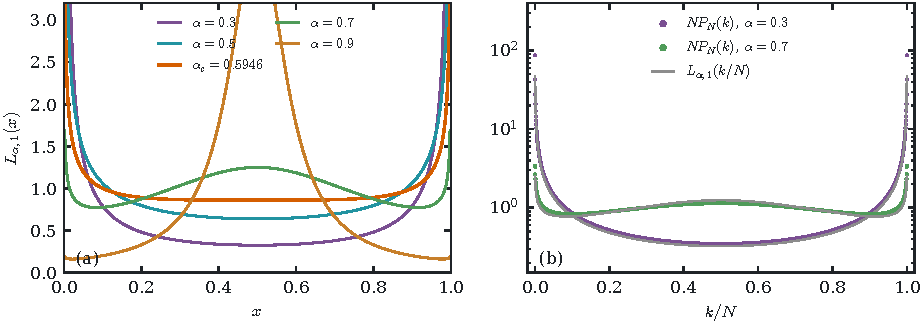
\includegraphics[width=\textwidth]{shape}
\caption{(a) The density $L_{\alpha,1}$ for $\alpha=0.3$, $0.5$, $\alpha_c$, $0.7$ and $0.9$.
At $\alpha_c$ the minimum at $1/2$ is flat to second order. (b) The exact law $NP_N(k)$ for
$N=2000$, the zeta law $f(n)\propto n^{-\alpha-1}$ for both signs and the fair start, with
$\alpha=0.3$ and $\alpha=0.7$, on a logarithmic scale, together with $L_{\alpha,1}(k/N)$. The
end values are of order $NT(N)$ and lie far above the density for $\alpha=0.3$.
Section~\ref{sec:verify} describes the computations.}
\label{fig:shape}
\end{figure} The discrete law $P_N$ has more structure near the ends. At distance
$j$ from the plus end it is the tail $T_\plus(N)$ times a renewal mass function
(Theorem~\ref{thm:ends}). Under Doney's condition this boundary layer matches the
bulk uniformly up to distance $o(N)$ from the end, and $NT_\plus(N)\to\infty$ makes
the end values much larger than the bulk values. So the global mode lies at bounded
distance from an end for every $\alpha\in(0,1)$ (Corollary~\ref{cor:mode}). For
$1<\alpha<2$ the same comparison has a golden ratio threshold~\cite{pemmasaniF}, and
here it has none. The ends also add local extrema of their own.
Theorem~\ref{thm:signs} gives a lower bound on the number of sign changes of
$k\mapsto P_N(k+1)-P_N(k)$, as the critical points of $\La$ plus the sign changes of
the two end profiles. Conjecture~\ref{conj:count} states that the bound is exact
for large $N$. It matches every case we computed.

\subsection{The initial run}\label{sec:intro-initial}

Wang, Schulz, Deng and Barkai~\cite{wsdb2018} studied renewal processes with
fat-tailed sojourn times in continuous time and left ``the effect of initial
preparation on the rare fluctuations'' for future work~\cite[Section~VIII]{wsdb2018}.
For the occupation count with $1<\alpha<2$ this is answered in~\cite{pemmasaniF}.
Theorem~\ref{thm:initial} treats $0<\alpha<1$. Let the first run have sign $\sgn$
and length $d$ with probability $\nu_\sgn(d)$. In the finite-mean case the bulk
needs no condition on the initial run on any macroscopic interior. Here it does.
A first run that ends just before the $k$-th plus step leaves a remainder that sits
in its own boundary layer, where the probabilities are of order $T(N)$ and not
$1/N$. Theorem~\ref{thm:initial} gives the exact defect in the bulk, the necessary
condition $\nu_\pm(n)=o(1/(nT_\plus(n)))$, the sufficient condition $n\nu_\pm(n)\to0$
under Doney's condition, and an exact criterion. It also shows by example that an
initial run which is finite almost surely can change the local law at interior
points, and that the necessary condition is not sufficient. At the ends the
criterion becomes the window condition
$\sum_{m<N/2}\nu_\plus(N-m)T_\plus(m)=o(T_\plus(N))$. Under Doney's condition every
fixed initial run with $n\nu_\pm(n)\to0$ leaves the local law and the end layers unchanged. An initial run
of length of order $N$ should change the local law itself, by an explicit mixture,
and we state this as Conjecture~\ref{rem:aging}.

\subsection{Related work}\label{sec:intro-related}

\emph{Occupation times.} Lamperti~\cite{lamperti1958} proved an occupation time
theorem for a class of stochastic processes, and the generalized arcsine density
$\La$ is attached to his name~\cite{margolinbarkai2006,zdk2015}. Mitov and
Yanev~\cite{mitovyanev2001} study limit theorems for the occupation-time process of
alternating renewal processes when the mean cycle is infinite, extending results of
Dynkin, Lamperti and Erickson for the spent lifetime. Starreveld, Bekker and
Mandjes~\cite{sbm2018} give the transform of the occupation time of an alternating
renewal process at an exponential time, a central limit theorem under finite second
moments, large deviations, and applications to L\'evy processes. Godr\`eche and
Luck~\cite{godrecheluck2001} give the transform of the occupation time and its limit
laws. All of these are statements in distribution. We found no local limit theorem
for the occupation count of an alternating renewal process with infinite means.

\emph{Strong renewal theorems.} The strong renewal theorem for $\alpha>1/2$ is due
to Garsia and Lamperti~\cite{garsialamperti1963}, Williamson~\cite{williamson1968}
and Erickson~\cite{erickson1970}. Doney~\cite{doney1997} proved it for all
$\alpha\in(0,1)$ under the local condition $f(n)=O(T(n)/n)$, together with a local
large deviation bound. Caravenna and Doney~\cite{caravennadoney2019} gave the
necessary and sufficient condition for $\alpha\le1/2$, and their local large
deviation bound for sums of a fixed number of variables is the main input of our
key estimate. Berger~\cite{berger2019ptrf} extends Doney's local bound, and his
version is the one we quote. Berger~\cite{berger2019} also proved multivariate
strong renewal theorems. Theorem~\ref{thm:local} shows that for the occupation count
the bivariate problem reduces exactly to the two univariate ones.

\emph{Physics.} In the physics literature the walk is the L\'evy walk in the ballistic
regime~\cite{zdk2015}, and the occupation count is the time average of a blinking
signal with power-law sojourn times~\cite{margolinbarkai2006}. Both sources use
$L_{\alpha,1}$ as the limit density of the time average. Wang, Schulz, Deng and
Barkai~\cite[Section~VII.A]{wsdb2018} found an atom with a boundary layer for the
occupation time when $0<\alpha<1$, for one sojourn law and a start of fair random
sign, through a double Laplace transform. Theorem~\ref{thm:ends} is a lattice
version of this layer at a fixed time, for two laws, with the uniform matching to
the bulk.

\emph{The finite-mean case.} For $1<\alpha<2$ the occupation law has a stable bulk,
big-jump zones and boundary layers, and its initial-run dependence and modes are
described in~\cite{pemmasaniF}. We use the exact identities of that paper and recall
them with proofs in Section~\ref{sec:identities}.

\emph{Organization.} Section~\ref{sec:setting} fixes notation and proves the exact
identities. Section~\ref{sec:tools} collects the cited theorems and proves the
elementary bounds, including the key estimate. Section~\ref{sec:local} proves
Theorem~\ref{thm:local}, Section~\ref{sec:shape} proves Theorem~\ref{thm:shape},
Section~\ref{sec:ends} treats the ends and the global mode, Section~\ref{sec:initial}
treats the initial run, and Section~\ref{sec:signs} counts sign changes.
Section~\ref{sec:verify} describes the computations. No proof uses a computed number.

\section{Setting, hypotheses and exact identities}\label{sec:setting}

\subsection{Runs and the occupation count}\label{sec:runs}

The walk takes $N$ steps and each step has a sign, $\plus$ or $\minus$. The signs
come in maximal runs of equal sign, and consecutive runs have opposite signs. All
runs after the first are independent. A run of sign $\sgn\in\{\plus,\minus\}$ has a
length distributed as $X_\sgn$, a random variable on $\{1,2,\dots\}$ with mass
function $f_\sgn(n)=\Prob(X_\sgn=n)$ and tail
\[
 T_\sgn(x)=\Prob(X_\sgn\ge x),\qquad x\in\R .
\]
We write $\osgn$ for the sign opposite to $\sgn$. The first run is the initial run.
It has a sign $\Sigma$ and a length $D$, the pair $(\Sigma,D)$ is independent of all
later runs, and $D<\infty$ almost surely. We put
\[
 \nu_\sgn(d)=\Prob(\Sigma=\sgn,\,D=d),\qquad Q_\sgn(N)=\Prob(\Sigma=\sgn,\,D\ge N),
 \qquad \pi_\sgn=\Prob(\Sigma=\sgn).
\]
Except in Conjecture~\ref{rem:aging}, the law of the initial run does not depend on
$N$. A fresh start of sign $\sgn_0$ has $\nu_{\sgn_0}=f_{\sgn_0}$ and
$\nu_{\osgn_0}=0$. The fair start is a fresh start of random sign, each sign with
probability $\frac12$.

Let $A_N$ be the number of plus steps among steps $1,\dots,N$, and
$P_N(k)=\Prob(A_N=k)$ for $0\le k\le N$. For a fresh start of sign $\sgn$ we write
$F^\sgn_N(k)$ for $P_N(k)$, with $F^\sgn_N(k)=0$ for $k\notin\{0,\dots,N\}$. We also
use
\[
 \Pi^\minus_m(j)=F^\minus_m(m-j),
\]
the probability that a fresh minus walk has exactly $j$ minus steps among its first
$m$ steps.

\subsection{Hypotheses}\label{sec:hypotheses}

The hypotheses carry fixed names, and every statement says which it uses.
\begin{itemize}[leftmargin=5em,labelsep=0.8em]
\item[(RV$_\alpha$)] $T_\plus$ is regularly varying with index $-\alpha$, where
$0<\alpha<1$, and $T_\minus(n)/T_\plus(n)\to b$ for some $b\in(0,\infty)$.
\item[(SPAN)] For each sign, the support of $X_\sgn$ is not contained in any
arithmetic progression $c+h\Z$ with $h\ge2$.
\item[(SRT$_\sgn$)] $u_\sgn(n)\sim\dfrac{\sin\pi\alpha}{\pi}\,\dfrac1{nT_\sgn(n)}$ as
$n\to\infty$, with $u_\sgn$ the renewal mass function of Section~\ref{sec:kernels}.
\item[(LB$_\sgn$)] There is $C$ with $f_\sgn(n)\le C\,T_\sgn(n)/n$ for all $n\ge1$.
\end{itemize}
Under (RV$_\alpha$) both tails are regularly varying with index $-\alpha$. Unequal
indices, or $b\in\{0,\infty\}$, give a degenerate limit of $A_N/N$ and are not
treated. (SPAN) is the aperiodicity needed for local limit theorems.
(SRT$_\sgn$) is the strong renewal theorem for the runs of sign $\sgn$. (LB$_\sgn$)
is Doney's local condition. It implies (SRT$_\sgn$) by Lemma~\ref{lem:cd}(iii)
below. A hypothesis written with the subscript $\pm$ is assumed for both signs.

\emph{Constants.} Unindexed $C$ and $c$ are positive constants that depend only on
the laws of the runs and may change from one use to the next. A constant written
$C_\delta$ also depends on $\delta$.

\subsection{Scales, stable densities and the Lamperti density}\label{sec:scales}

Under (RV$_\alpha$) choose an increasing function $a:(0,\infty)\to(0,\infty)$ with
$t\,T_\plus(a(t))\to1$ as $t\to\infty$, and put $a_m=a(m)$. So $a$ is regularly
varying with index $1/\alpha$. For $t>0$ let
\[
 m_N(t)=\lfloor t/T_\plus(N)\rfloor .
\]
Then $T_\plus(a_{m_N(t)})\sim T_\plus(N)/t$, and $a_{m_N(t)}/N\to t^{1/\alpha}$ uniformly for $t$
in compact subsets of $(0,\infty)$ (Lemma~\ref{lem:rv-facts}).

Put $\Gam=\Gamma(1-\alpha)$, and let $g$ be the density of the positive stable
variable $Z$ with $\E e^{-\lambda Z}=e^{-\Gam\lambda^\alpha}$. Its L\'evy measure is
$\alpha r^{-\alpha-1}dr$ on $(0,\infty)$, with tail $r^{-\alpha}$. For $t>0$ let
\[
 p_t(z)=t^{-1/\alpha}g\bigl(zt^{-1/\alpha}\bigr),
\]
the density at time $t$ of the stable subordinator with Laplace exponent
$t\Gam\lambda^\alpha$. The covering densities are
\begin{equation}\label{eq:covering}
 Q_t(x)=\int_0^xp_t(z)(x-z)^{-\alpha}\,dz,\qquad
 Q^b_t(y)=b\int_0^yp_{bt}(z)(y-z)^{-\alpha}\,dz .
\end{equation}
The density $g$ is continuous and bounded, and $g(w)\sim\alpha w^{-1-\alpha}$ as
$w\to\infty$~\cite[Section~XVII.6]{feller1971}. Hence
\begin{equation}\label{eq:p-bound}
 p_t(z)\le C\min\bigl\{t^{-1/\alpha},\,t\,z^{-1-\alpha}\bigr\}\qquad(t,z>0).
\end{equation}
For $0<x<1$ let
\begin{equation}\label{eq:Lambda}
 \Lambda(x)=\int_0^\infty\bigl[p_{bt}(1-x)\,Q_t(x)+p_t(x)\,Q^b_t(1-x)\bigr]\,dt .
\end{equation}
The Lamperti density $\La$ is defined in~\eqref{eq:lamperti-intro}. With
$t=\log((1-x)/x)$ and $\beta=\log b$ it reads
\begin{equation}\label{eq:L-cosh}
 \La(x)=\frac{\sin\pi\alpha}{\pi}\,\frac{1+\cosh t}{\cosh(\alpha t-\beta)+\cos\pi\alpha}.
\end{equation}
To check~\eqref{eq:L-cosh}, write $w=(1-x)/x=e^t$. Then
$x^{\alpha-1}(1-x)^{\alpha-1}=x^{2\alpha-2}w^{\alpha-1}$, the denominator
of~\eqref{eq:lamperti-intro} is $x^{2\alpha}bw^\alpha\cdot2[\cosh(\alpha t-\beta)+\cos\pi\alpha]$,
and $x^{-2}w^{-1}=(1+w)^2/w=2+2\cosh t$. We also use, for $0\le y<1$,
\begin{equation}\label{eq:Phi}
 \Phi_b(y)=\frac{b^2(1-y)^{\alpha-1}}{b^2(1-y)^{2\alpha}+2b\cos(\pi\alpha)\,(1-y)^\alpha y^\alpha+y^{2\alpha}},
\end{equation}
so $\Phi_b(0)=1$, $\Phi_b(y)=1+O(y^\alpha)$ as $y\to0$, $\Phi_b>0$, and
$\La(1-y)=\frac{\sin\pi\alpha}{\pi b}\,y^{\alpha-1}\Phi_b(y)$.

\subsection{Renewal kernels}\label{sec:kernels}

For each sign let $X^\sgn_1,X^\sgn_2,\dots$ be independent copies of $X_\sgn$,
$S^\sgn_m=X^\sgn_1+\dots+X^\sgn_m$ with $S^\sgn_0=0$, and $u^\sgn_m=f_\sgn^{*m}$ the
law of $S^\sgn_m$, so $u^\sgn_0=\delta_0$. The renewal mass function is
\[
 u_\sgn(j)=\sum_{m\ge0}u^\sgn_m(j),\qquad j\ge0,
\]
so $u_\sgn(0)=1$. For $m\ge1$ and $k\ge1$ let
\begin{equation}\label{eq:q-cover}
 q^\sgn_m(k)=\Prob\bigl(S^\sgn_{m-1}<k\le S^\sgn_m\bigr)=\sum_{r<k}u^\sgn_{m-1}(r)\,T_\sgn(k-r),
\end{equation}
the probability that the $m$-th run of sign $\sgn$ covers level $k$ in the time of
its sign. The second form holds because $X^\sgn_m$ is independent of $S^\sgn_{m-1}$.
For each $k\ge1$ exactly one $m$ has $S^\sgn_{m-1}<k\le S^\sgn_m$, so
$\sum_{m\ge1}q^\sgn_m(k)=1$. We write $\omega_\sgn(i)=\min\{1,1/(iT_\sgn(i))\}$ for
$i\ge1$ and $\omega_\sgn(0)=1$. Under (SRT$_\sgn$) we have $u_\sgn\le C\omega_\sgn$.

\subsection{Exact identities}\label{sec:identities}

The following identities hold for every $N$ and need no hypothesis. They are
proved in~\cite[Section~2]{pemmasaniF}, and we include the short proofs. The
computations of Section~\ref{sec:verify} check them against a sum over all sign
strings.

\begin{proposition}[the fresh-plus identity]\label{prop:fresh-identity}
For $k,j\ge1$ with $k+j=N$,
\begin{equation}\label{eq:fresh}
 F^\plus_N(k)=\sum_{m\ge1}u^\minus_m(j)\,q^\plus_{m+1}(k)+\sum_{m\ge1}u^\plus_m(k)\,q^\minus_m(j),
\end{equation}
and $F^\plus_N(N)=T_\plus(N)$, $F^\plus_N(0)=0$. Exchanging the signs, for $k,j\ge1$,
$F^\minus_N(k)=\sum_{m\ge1}[u^\plus_m(k)q^\minus_{m+1}(j)+u^\minus_m(j)q^\plus_m(k)]$,
with $F^\minus_N(0)=T_\minus(N)$ and $F^\minus_N(N)=0$.
\end{proposition}

\begin{proof}
For a fresh plus start the $i$-th plus run fills the steps in
$(S^\plus_{i-1}+S^\minus_{i-1},\,S^\plus_i+S^\minus_{i-1}]$ and the $i$-th minus run
fills those in $(S^\plus_i+S^\minus_{i-1},\,S^\plus_i+S^\minus_i]$. These intervals
partition $\{1,2,\dots\}$. If step $N$ lies in the $i$-th plus run, the first $N$
steps contain exactly $S^\minus_{i-1}$ minus steps. So $A_N=k$ means
$S^\minus_{i-1}=j$, and then step $N$ lies in that run exactly when
$S^\plus_{i-1}<k\le S^\plus_i$. The two events concern independent sequences, so
this case has probability $u^\minus_{i-1}(j)q^\plus_i(k)$. If step $N$ lies in the
$i$-th minus run, then $A_N=k$ means $S^\plus_i=k$, and step $N$ lies in that run
exactly when $S^\minus_{i-1}<j\le S^\minus_i$, with probability
$u^\plus_i(k)q^\minus_i(j)$. The cases are disjoint. For $j\ge1$ the plus case with
$i=1$ vanishes, and $m=i-1$ in the plus case and $m=i$ in the minus case
give~\eqref{eq:fresh}. For $k=N$ only the plus case with $i=1$ survives, with
probability $T_\plus(N)$, and $k=0$ is impossible. The fresh minus start is the same
with the signs exchanged.
\end{proof}

\begin{proposition}[the first-run decomposition]\label{prop:first-run}
For every initial run and every $0\le k\le N$,
\[
 P_N(k)=Q_\plus(N)\ones_{\{k=N\}}+Q_\minus(N)\ones_{\{k=0\}}
 +\sum_{d<N}\nu_\plus(d)\,F^\minus_{N-d}(k-d)+\sum_{d<N}\nu_\minus(d)\,F^\plus_{N-d}(k).
\]
In particular $P_N(N)=Q_\plus(N)$ and $P_N(0)=Q_\minus(N)$.
\end{proposition}

\begin{proof}
We condition on the initial run. If $\Sigma=\plus$ and $D\ge N$, then $A_N=N$. If
$\Sigma=\plus$ and $D=d<N$, steps $d+1,\dots,N$ are the first $N-d$ steps of a fresh
minus walk independent of $(\Sigma,D)$, so $A_N=d+A'$ with $A'$ of law
$F^\minus_{N-d}$. The case $\Sigma=\minus$ is the same. For $d<N$
Proposition~\ref{prop:fresh-identity} gives $F^\minus_{N-d}(N-d)=0$ and
$F^\plus_{N-d}(0)=0$, so only the atoms survive at $k=N$ and $k=0$.
\end{proof}

\begin{proposition}[the final-run identity]\label{prop:final-run}
For a fresh plus start, $N\ge1$ and $0\le j<N$,
\begin{equation}\label{eq:final-explicit}
\begin{split}
 P_N(N-j)={}&\sum_{r=0}^{j}u^\minus_r(j)\,\E\bigl[T_\plus(N-j-S^\plus_r);\,S^\plus_r\le N-j-1\bigr]\\
 &+\sum_{m=1}^{j}T_\minus(m)\sum_{r=0}^{j-m}u^\minus_r(j-m)\,u^\plus_{r+1}(N-j).
\end{split}
\end{equation}
\end{proposition}

\begin{proof}
We split according to the run that contains step $N$, the final run. The
$(r+1)$-th plus run starts at step $S^\plus_r+S^\minus_r+1$. It is the final run and
$A_N=N-j$ exactly when $S^\minus_r=j$ and $X^\plus_{r+1}\ge N-j-S^\plus_r\ge1$. This
gives the term $r$ of the first sum. The $(r+1)$-th minus run starts at step
$S^\plus_{r+1}+S^\minus_r+1$. If it is the final run and starts at step $N-m+1$, then
$A_N=N-j$ means $S^\plus_{r+1}=N-j$ and $S^\minus_r=j-m$, which needs $1\le m\le j$,
and $X^\minus_{r+1}\ge m$. This gives the second sum. Exactly one run is final, and
$u^\minus_r(i)=0$ for $r>i$.
\end{proof}

For the computations we use a third form of the law. For a fresh plus start let
$A(k,j)$ and $B(k,j)$ be the probabilities that a plus run, respectively a minus run,
starts right after exactly $k$ plus steps and $j$ minus steps. A plus run is preceded
by $m$ runs of each sign and a minus run by $m$ plus runs and $m-1$ minus runs, so
\[
 A(k,j)=\sum_{m\ge0}u^\plus_m(k)u^\minus_m(j),\qquad B(k,j)=\sum_{m\ge1}u^\plus_m(k)u^\minus_{m-1}(j).
\]
Splitting on the start of the final run gives, with $j=N-k$,
\begin{equation}\label{eq:run-sum}
 F^\plus_N(k)=\sum_{k'<k}A(k',j)\,T_\plus(k-k')+\sum_{j'<j}B(k,j')\,T_\minus(j-j').
\end{equation}
Every term is nonnegative.

\section{Tools}\label{sec:tools}

\subsection{Regular variation}\label{sec:rv}

We use the following facts about a function $T$ that is regularly varying with
index $-\alpha\in(-1,0)$, all from~\cite[Sections~1.2 to~1.5]{bgt1989}.
\begin{enumerate}[(R1)]
\item (Uniform convergence.) $T(\lambda x)/T(x)\to\lambda^{-\alpha}$ uniformly for
$\lambda$ in compact subsets of $(0,\infty)$.
\item (Potter.) For every $c\ge1$ there is $C_c$ with $T(x/c)\le C_cT(x)$ for $x\ge c$.
\item (Karamata.) $\sum_{n\le w}T(n)\sim wT(w)/(1-\alpha)$ and
$\sum_{1\le i\le w}1/(iT(i))\sim1/(\alpha T(w))$ as $w\to\infty$.
\item (Dyadic sums.) $\sum_{l\ge1,\,2^l\le x}2^lT(2^{l-1})\le CxT(x)$ and
$\sum_{l\ge1,\,2^l>x}T(2^{l-1})\le CT(x)$ for $x\ge1$.
\end{enumerate}
(R4) follows from (R2) and Potter's theorem~\cite[Theorem~1.5.6]{bgt1989}, since $wT(w)$ is regularly varying with the
positive index $1-\alpha$ and $T$ with the negative index $-\alpha$, so both sums are
dominated by geometric series (Lemma~\ref{lem:rv-facts}). Under (RV$_\alpha$) the two tails are comparable,
$c\,T_\plus\le T_\minus\le C\,T_\plus$, and $mT_\plus(a_m)\le C$ for all $m\ge1$. We
also use $a_{\lceil m/3\rceil}\ge c\,a_m$, which follows from (R2) for the function
$a$.

\subsection{Cited theorems}\label{sec:cited}

Under (RV$_\alpha$) and (SPAN), $S^\plus_m/a_m$ converges in law to $Z$, and
$S^\minus_m/a_m$ converges to $b^{1/\alpha}Z$, whose density is
$g_b(z)=b^{-1/\alpha}g(zb^{-1/\alpha})$. Note that $t^{-1/\alpha}g_b(yt^{-1/\alpha})=p_{bt}(y)$.

\begin{lemma}[classical inputs]\label{lem:cd}
Assume (RV$_\alpha$) and (SPAN).
\begin{enumerate}[(i)]
\item (Gnedenko's local limit theorem~\cite[Theorem~4.2.1]{ibragimovlinnik1971}.)
$\sup_x|a_mu^\plus_m(x)-g(x/a_m)|\to0$ and $\sup_y|a_mu^\minus_m(y)-g_b(y/a_m)|\to0$ as
$m\to\infty$. Hence $\sup_xu^\sgn_m(x)\le C/a_m$ for all $m\ge1$ and both signs.
\item (Local large deviations~\cite[Theorem~1.1, Eq.~(1.6)]{caravennadoney2019}.)
For both signs there is $C$ with $u^\sgn_m(x)\le C\,\dfrac m{a_m}\,T_\sgn(x)$ for all
$m\ge1$ and $x\ge1$.
\item (The strong renewal theorem.) If $\alpha>1/2$, (SRT$_\sgn$) holds for both signs
\cite{garsialamperti1963,erickson1970}, see~\cite[Theorem~1.4]{caravennadoney2019}.
If $\alpha\le1/2$, (SRT$_\sgn$) holds if and only if
\[
 \lim_{\delta\to0}\limsup_{x\to\infty}\,xT_\sgn(x)\sum_{1\le z\le\delta x}
 \frac{f_\sgn(x-z)}{zT_\sgn(z)^2}=0
\]
\cite[Theorem~1.4]{caravennadoney2019}. In every case (LB$_\sgn$) implies
(SRT$_\sgn$)~\cite{doney1997}, see~\cite[Eq.~(1.15)]{caravennadoney2019}.
\item (The strong renewal theorem as a small-$m$ condition~\cite[Section~4.1,
Eq.~(4.1)]{caravennadoney2019}.) For each sign, (SRT$_\sgn$) holds if and only if
\begin{equation}\label{eq:cd41}
 \lim_{\delta\to0}\limsup_{x\to\infty}I_\sgn(\delta,x)=0,\qquad
 I_\sgn(\delta,x)=xT_\sgn(x)\sum_{1\le m\le\delta/T_\sgn(x)}u^\sgn_m(x).
\end{equation}
\item (Doney's local bound~\cite[Theorem~2.4]{berger2019ptrf}, extending~\cite[Theorem~A]{doney1997}.)
Under (LB$_\sgn$) there is $C$ with $u^\sgn_m(x)\le C\,mT_\sgn(x)/x$ for all $m\ge1$
and $x\ge a_m$.
\end{enumerate}
\end{lemma}

We comment on the form of these statements. In (ii) and (iv) Caravenna and Doney
use the tail $\Prob(X>x)$ and a function $A$ with $A(x)\sim1/\Prob(X>x)$ for renewal
laws. The difference between $\Prob(X>x)$ and $T(x)=\Prob(X\ge x)$ is
$f(x)=o(T(x))$. In (iv) their condition reads
$\lim_{\delta\to0}\limsup_x(x/A(x))\sum_{1\le m\le A(\delta x)}u_m(x)=0$. Since
$A(\delta x)\sim\delta^\alpha/T(x)$ and the sum increases with its upper limit, this
is equivalent to~\eqref{eq:cd41}. (SPAN) makes the span $1$, so their
$\Prob(S_m\in x+(-1,0])$ is $u_m(x)$. In (v) Berger uses a scale $a'_m$ that may differ
from ours by a constant factor. For $c\,a_m\le x\le a_m$ the bound follows from (ii),
since $m/a_m\le m/x$ there, so (v) holds for $x\ge a_m$ with our scale.

\subsection{Elementary bounds}\label{sec:elementary}

The following bounds use only (RV$_\alpha$) and (SPAN). We state them for the plus
sign and they hold for the minus sign with the same proofs. We drop the sign from
the notation.

\begin{lemma}[sums of runs]\label{lem:sums}
\begin{enumerate}[(i)]
\item $\Prob(S_m\ge x)\le C\,mT(x)$ for all $m,x\ge1$.
\item $\Prob(S_m<x)\le e^{-mT(x)}$ for all $m\ge0$ and $x\ge1$.
\item $u_m(x)\le C\,a_m^{-1}e^{-mT(x+1)/3}$ for all $m\ge2$ and $x\ge0$.
\end{enumerate}
\end{lemma}

\begin{proof}
(i) If $S_m\ge x$, then some $X_i\ge x$, or $\sum_iX_i\ones_{\{X_i<x\}}\ge x$. By the
union bound and Markov's inequality,
$\Prob(S_m\ge x)\le mT(x)+m\,\E[X;X<x]/x$. Now
$\E[X;X<x]=\sum_{1\le n<x}\Prob(n\le X<x)\le\sum_{n<x}T(n)\le CxT(x)$ by (R3).

(ii) $S_m<x$ forces $X_i<x$ for every $i\le m$, which has probability
$(1-T(x))^m\le e^{-mT(x)}$.

(iii) Let $h=\lfloor m/2\rfloor\ge m/3$. Conditioning on $S_h$,
$u_m(x)=\sum_{y\le x}u_h(y)u_{m-h}(x-y)\le\Prob(S_h\le x)\sup_zu_{m-h}(z)$. By (ii)
$\Prob(S_h\le x)=\Prob(S_h<x+1)\le e^{-mT(x+1)/3}$, and by Lemma~\ref{lem:cd}(i)
$\sup_zu_{m-h}(z)\le C/a_{m-h}\le C/a_m$, since $m-h\ge m/2$.
\end{proof}

\begin{lemma}[the covering kernel at scale $N$]\label{lem:kernel-limit}
Fix $\delta\in(0,1)$. Uniformly for $t\in[\delta,1/\delta]$ and $x\in[\delta,1]$,
\[
 q^\plus_{m_N(t)+1}(\lfloor xN\rfloor)=T_\plus(N)\bigl[Q_t(x)+o(1)\bigr],\qquad
 q^\minus_{m_N(t)}(\lfloor xN\rfloor)=T_\plus(N)\bigl[Q^b_t(x)+o(1)\bigr].
\]
\end{lemma}

\begin{proof}
Write $m=m_N(t)$ and $k=\lfloor xN\rfloor$, and fix $\theta\in(0,\delta/2)$. Split
$q^\plus_{m+1}(k)=\sum_{r<k}u^\plus_m(r)T_\plus(k-r)$ at $r=k-\theta N$. On
$r\le k-\theta N$ we have $(k-r)/N\in[\theta,1]$, so by (R1)
$T_\plus(k-r)/T_\plus(N)=((k-r)/N)^{-\alpha}+o(1)$ uniformly. By
Lemma~\ref{lem:cd}(i), $u^\plus_m(r)=a_m^{-1}[g(r/a_m)+o(1)]$ uniformly in $r$. The error
terms contribute at most $o(1/a_m)\cdot k\cdot T_\plus(\theta N)=o(T_\plus(N))$, since
$N/a_m$ is bounded. The main term is
$T_\plus(N)\sum_{r\le k-\theta N}a_m^{-1}g(r/a_m)((k-r)/N)^{-\alpha}$, a Riemann sum with mesh
$1/N$ in $z=r/N$. Since $a_m/N\to t^{1/\alpha}$ uniformly and $g$ is bounded and uniformly
continuous, it converges to $\int_0^{x-\theta}p_t(z)(x-z)^{-\alpha}dz$, uniformly in
$t$ and $x$. On $r>k-\theta N$, Lemma~\ref{lem:cd}(i) and (R3) give at most
$(C/a_m)\sum_{i<\theta N+1}T_\plus(i)\le C_\delta\,\theta^{(1-\alpha)/2}T_\plus(N)$ for large
$N$, using (R1) and (R2) to compare $\theta NT_\plus(\theta N)$ with $NT_\plus(N)$. By the
first bound in~\eqref{eq:p-bound} the integral over $[x-\theta,x]$ is at most
$C_\delta\theta^{1-\alpha}$. Let $N\to\infty$ and then $\theta\to0$. The minus kernel is the
same with $u^\minus_{m-1}$ in place of $u^\plus_m$, the density $g_b$ in place of $g$,
and $T_\minus(N)\sim bT_\plus(N)$. The shift from $m$ to $m-1$ does not change the
limit.
\end{proof}

The next bound is the key estimate of the paper. It bounds the covering kernel by
the tail at the level, uniformly in the number of runs, under regular variation
alone.

\begin{lemma}[the key bound]\label{lem:key}
For both signs there is $C$ with $q^\sgn_{m+1}(k)\le C\,T_\sgn(k)$ for all $m\ge0$ and
$k\ge1$.
\end{lemma}

\begin{proof}
We drop the sign. For $m=0$, $q_1=T$. Let $m\ge1$. By~\eqref{eq:q-cover},
$q_{m+1}(k)=\sum_{r<k}u_m(r)T(k-r)$. The part with $r<k/2$ is at most
$T(k/2)\le CT(k)$ by (R2). For $r\ge k/2$ put $i=k-r\in[1,k/2]$, and split the range
of $i$ into dyadic blocks $[w/2,w)$ with $w=2^l$, $l\ge1$, $w\le k$. On a block,
\[
 \sum_{w/2\le i<w}u_m(k-i)T(i)\le T(w/2)\,\Prob\bigl(S_m\in(k-w,k-w/2]\bigr).
\]
The window has at most $w$ lattice points, all at least $k/2$. By
Lemma~\ref{lem:cd}(ii) and (R2) each point has probability at most
$C(m/a_m)T(k)$. By Lemma~\ref{lem:sums}(i) and (R2) the whole window has probability
at most $C\,mT(k)$. So the block is at most
$C\,mT(k)\,T(w/2)\min\{1,w/a_m\}$. Summing with (R4), the blocks with $w\le a_m$ give
at most $C\frac{mT(k)}{a_m}\sum_{w\le a_m}wT(w/2)\le C\,mT(k)T(a_m)$, and the blocks
with $w>a_m$ give at most $C\,mT(k)\sum_{w>a_m}T(w/2)\le C\,mT(k)T(a_m)$. Since
$mT(a_m)\le C$, the total is at most $CT(k)$.
\end{proof}

Note that Lemma~\ref{lem:cd}(ii) is used here at points $x\ge k/2$ that may lie far
below $a_m$ as well as above it, and it holds for all $x$.

\begin{lemma}[decay in $m$]\label{lem:decay}
For both signs there are $C,c$ with $q^\sgn_m(j)\le C\,T_\sgn(j)\,e^{-c\,mT_\sgn(j)}$ for
all $m,j\ge1$.
\end{lemma}

\begin{proof}
We drop the sign. If $mT(j)\le9$, this is Lemma~\ref{lem:key} with $c=1/9$. Let
$mT(j)>9$, so $m\ge10$, and put $h=\lfloor(m-1)/2\rfloor\ge m/3$. Splitting
$S_{m-1}=S_h+(S_{m-1}-S_h)$ gives $q_m(j)=\sum_{s<j}u_h(s)\,q_{m-h}(j-s)$. For $s<j/2$
we use $q_{m-h}(j-s)\le CT(j-s)\le CT(j)$ (Lemma~\ref{lem:key} and (R2)) and
$\Prob(S_h<j/2)\le e^{-hT(j)}\le e^{-mT(j)/3}$ (Lemma~\ref{lem:sums}(ii)). For
$j/2\le s<j$ we use
\[
 \sum_{j/2\le s<j}u_h(s)\,q_{m-h}(j-s)\le\sup_{s<j}u_h(s)\sum_{i\le j/2}CT(i)
 \le C\,a_h^{-1}e^{-hT(j)/3}\,jT(j),
\]
by Lemma~\ref{lem:sums}(iii) and (R3). Since $hT(j)\ge mT(j)/3>3$, we have
$T(j)\ge3/h\ge T(a_h)$ for large $h$, so $j\le Ca_h$ and $jT(j)/a_h\le CT(j)$. Both
parts are at most $CT(j)e^{-mT(j)/9}$.
\end{proof}

\section{The local Lamperti law}\label{sec:local}

\subsection{The limit density}\label{sec:lamperti}

\begin{proposition}[identification of the limit]\label{prop:lambda}
The integral $\Lambda$ of~\eqref{eq:Lambda} is finite and continuous on $(0,1)$, and
$\Lambda=\La$. Moreover, for every $\theta>-1$,
\begin{equation}\label{eq:stieltjes}
 \int_0^1\frac{\La(v)\,dv}{1+\theta v}=\frac{(1+\theta)^{\alpha-1}+b}{(1+\theta)^\alpha+b},
\end{equation}
so $\La$ is a probability density with mean $1/(1+b)$.
\end{proposition}

\begin{proof}
\emph{Finiteness and continuity.} Let $x$ range over a compact subset $K$ of $(0,1]$.
Split $Q_t(x)$ at $z=x/2$. The part $z<x/2$ is at most $(x/2)^{-\alpha}$, and by
\eqref{eq:p-bound} the part $z\ge x/2$ is at most
$C\min\{t^{-1/\alpha},t\}\int_0^{x/2}w^{-\alpha}dw$. So
$Q_t(x)\le C_K(1+\min\{t^{-1/\alpha},t\})$, and the same holds for $Q^b_t$.
By~\eqref{eq:p-bound}, $p_t(x)\le C_K\min\{t^{-1/\alpha},t\}$. The integrand
of~\eqref{eq:Lambda} is therefore at most $C_K\min\{t^{-1/\alpha},t\}$ for $x\in K$,
which is integrable on $(0,\infty)$ because $1/\alpha>1$. The integrand is
continuous in $x$, so $\Lambda$ is finite and continuous by dominated convergence.

\emph{Homogeneity.} For $x,y>0$ put
$\lambda(x,y)=\int_0^\infty[p_{bt}(y)Q_t(x)+p_t(x)Q^b_t(y)]\,dt$, so
$\Lambda(x)=\lambda(x,1-x)$. For $c>0$ the definitions give
$p_t(cz)=c^{-1}p_{tc^{-\alpha}}(z)$, and the substitution $z=cw$ in~\eqref{eq:covering}
gives $Q_t(cx)=c^{-\alpha}Q_{tc^{-\alpha}}(x)$ and $Q^b_t(cy)=c^{-\alpha}Q^b_{tc^{-\alpha}}(y)$.
Substituting $s=tc^{-\alpha}$ in the integral over $t$ then gives
$\lambda(cx,cy)=c^{-1}\lambda(x,y)$. Hence
\[
 \lambda(x,y)=\frac1{x+y}\,\Lambda\Bigl(\frac x{x+y}\Bigr).
\]

\emph{The double Laplace transform.} For $\lambda,\mu>0$,
$\int_0^\infty e^{-\mu y}p_{bt}(y)\,dy=e^{-bt\Gam\mu^\alpha}$, and since $Q_t$ is the
convolution of $p_t$ with $w^{-\alpha}$ on $(0,\infty)$,
\[
 \int_0^\infty e^{-\lambda x}Q_t(x)\,dx=e^{-t\Gam\lambda^\alpha}\,\Gam\lambda^{\alpha-1},\qquad
 \int_0^\infty e^{-\mu y}Q^b_t(y)\,dy=b\,e^{-bt\Gam\mu^\alpha}\,\Gam\mu^{\alpha-1}.
\]
All functions are nonnegative, so by Tonelli's theorem
\[
 \int_0^\infty\!\!\int_0^\infty e^{-\lambda x-\mu y}\lambda(x,y)\,dx\,dy
 =\int_0^\infty\Gam\bigl(\lambda^{\alpha-1}+b\mu^{\alpha-1}\bigr)e^{-t\Gam(\lambda^\alpha+b\mu^\alpha)}\,dt
 =\frac{\lambda^{\alpha-1}+b\mu^{\alpha-1}}{\lambda^\alpha+b\mu^\alpha}.
\]
Now change variables to $x=sv$, $y=s(1-v)$ with $s>0$ and $v\in(0,1)$, so
$dx\,dy=s\,ds\,dv$. By homogeneity the left side is
\[
 \int_0^1\Lambda(v)\int_0^\infty e^{-s(\lambda v+\mu(1-v))}\,ds\,dv
 =\int_0^1\frac{\Lambda(v)\,dv}{\lambda v+\mu(1-v)} .
\]
With $\mu=1$ and $\lambda=1+\theta$ this is~\eqref{eq:stieltjes} with $\Lambda$ in place of
$\La$. At $\theta=0$ it gives $\int_0^1\Lambda=1$.

\emph{Inversion.} For $z\in\C\setminus[0,1]$ let
$G(z)=\int_0^1\Lambda(v)\,dv/(z-v)$, and let
$H(w)=(w^{\alpha-1}+b)/(w^\alpha+b)$ with principal powers on
$\C\setminus(-\infty,0]$. The denominator does not vanish there, since
$|\arg w^\alpha|<\pi\alpha<\pi$. For real $z>1$ put $\theta=-1/z\in(-1,0)$. Then
$1/(z-v)=z^{-1}/(1+\theta v)$, so the transform gives $G(z)=z^{-1}H(1-1/z)$. Since
$1-1/z\in(-\infty,0]$ exactly when $z\in(0,1]$, the right side is analytic on
$\C\setminus[0,1]$, as is $G$. The two agree on $(1,\infty)$, hence on all of
$\C\setminus[0,1]$. Since $\Lambda$ is continuous and integrable,
$-\frac1\pi\mathrm{Im}\,G(x+i\varepsilon)$ tends to $\Lambda(x)$ as $\varepsilon\downarrow0$ for
every $x\in(0,1)$ (Lemma~\ref{lem:poisson}).

We compute the boundary value. Let $x\in(0,1)$ and $w=(1-x)/x$. As
$\varepsilon\downarrow0$, $1-1/(x+i\varepsilon)$ tends to $-w$ from the upper half
plane, so it tends to $we^{i\pi}$ on the principal branch. With $E=e^{i\pi\alpha}$ this
gives $(we^{i\pi})^\alpha=w^\alpha E$ and $(we^{i\pi})^{\alpha-1}=-w^{\alpha-1}E$, so
\[
 G(x+i0)=\frac1x\,\frac{b-w^{\alpha-1}E}{b+w^\alpha E}
 =\frac1x\,\frac{(b-w^{\alpha-1}E)(b+w^\alpha\bar E)}{b^2+2bw^\alpha\cos\pi\alpha+w^{2\alpha}} .
\]
The imaginary part of the numerator is $-b\sin(\pi\alpha)\,w^{\alpha-1}(1+w)$. Hence
\[
 -\frac1\pi\,\mathrm{Im}\,G(x+i0)=\frac{\sin\pi\alpha}\pi\,
 \frac{b\,w^{\alpha-1}(1+w)}{x\,(b^2+2bw^\alpha\cos\pi\alpha+w^{2\alpha})}.
\]
Since $1+w=1/x$, we have $w^{\alpha-1}(1+w)/x=x^{-1-\alpha}(1-x)^{\alpha-1}$, and the
denominator is $x^{-2\alpha}[b^2x^{2\alpha}+2b\cos(\pi\alpha)x^\alpha(1-x)^\alpha+(1-x)^{2\alpha}]$.
So the right side is $\La(x)$, and $\Lambda=\La$. Finally, differentiating
\eqref{eq:stieltjes} at $\theta=0$ gives $-\int_0^1v\La(v)\,dv=-1/(1+b)$.
\end{proof}

The mean $1/(1+b)$ has the expected direction. If $b<1$, the plus runs are heavier
and the plus steps occupy more than half of the time on average.

\subsection{Proof of Theorem~\ref{thm:local}}\label{sec:local-proof}

We first describe the structure of the proof. By the fresh-plus identity, $P_N(k)$ is a sum
over the number $m$ of completed minus runs (first sum) or plus runs (second sum) of a product
of a point probability and a covering probability. Typical configurations have $m$ of order
$1/T_\plus(N)$, since $m$ runs of a law with tail $T$ have total length of order $a_m$, and
$a_m\asymp N$ exactly when $mT_\plus(N)\asymp1$. On this range Gnedenko's theorem and
Lemma~\ref{lem:kernel-limit} turn the sum into a Riemann sum for $\Lambda$. Large $m$ is
negligible because $N$ steps rarely contain many more runs than $1/T(N)$, which is
Lemma~\ref{lem:sums}(iii). Small $m$ is the delicate range. There a few runs have total length
of order $N$, so one run is of order $N$, and the probability that a sum of few runs lands
exactly on a given point is the quantity controlled by the strong renewal theorem. The key
bound of Lemma~\ref{lem:key} removes the covering probability from this range at the cost of a
constant, and Lemma~\ref{lem:cd}(iv) then says that what is left is negligible if and only if
the strong renewal theorem holds. Since every term is nonnegative, the same comparison runs in
the other direction and gives the necessity.

We prove the theorem for a fresh plus start. Fix
$0<x_1<x_2<1$ and let $k$ range over $[x_1N,x_2N]$. Put $j=N-k$, $x=k/N$ and $y=1-x$.
By Proposition~\ref{prop:fresh-identity},
\[
 P_N(k)=\underbrace{\sum_{m\ge1}u^\minus_m(j)\,q^\plus_{m+1}(k)}_{\mathrm{I}}
 +\underbrace{\sum_{m\ge1}u^\plus_m(k)\,q^\minus_m(j)}_{\mathrm{II}}.
\]
Every term is nonnegative. Fix $\delta\in(0,1)$ and split the sums over $m$ into small
$m<\delta/T_\plus(N)$, medium $\delta/T_\plus(N)\le m\le1/(\delta T_\plus(N))$ and large
$m>1/(\delta T_\plus(N))$. We write $\mathrm I_{\rm s}$, $\mathrm I_{\rm m}$, $\mathrm I_{\rm l}$
and so on. Let
\[
 \Lambda_\delta(x)=\int_\delta^{1/\delta}\bigl[p_{bt}(1-x)Q_t(x)+p_t(x)Q^b_t(1-x)\bigr]\,dt .
\]
By Proposition~\ref{prop:lambda}, $\Lambda_\delta$ increases to $\La$ as $\delta\to0$, and
by Dini's theorem the convergence is uniform on $[x_1,x_2]$.

\emph{Medium $m$.} Every medium $m$ is $m_N(t)$ for $t=mT_\plus(N)\in[\delta,1/\delta]$, and
$a_m=Nt^{1/\alpha}(1+o(1))$ uniformly. By Lemma~\ref{lem:cd}(i),
$Nu^\minus_m(j)=p_{bt}(y)+o(1)$ and $Nu^\plus_m(k)=p_t(x)+o(1)$ uniformly. By
Lemma~\ref{lem:kernel-limit}, $q^\plus_{m+1}(k)=T_\plus(N)[Q_t(x)+o(1)]$ and
$q^\minus_m(j)=T_\plus(N)[Q^b_t(y)+o(1)]$ uniformly. Put
$h(t,x)=p_{bt}(1-x)Q_t(x)+p_t(x)Q^b_t(1-x)$. Since $p_t$, $Q_t$ and $Q^b_t$ are bounded on
the relevant compact sets, the products of the error terms are $o(1)$ uniformly, so
\[
 N(\mathrm I_{\rm m}+\mathrm{II}_{\rm m})=\sum_{\delta/T_\plus(N)\le m\le1/(\delta T_\plus(N))}
 T_\plus(N)\bigl[h(mT_\plus(N),x)+o(1)\bigr].
\]
The number of terms is at most $1/(\delta T_\plus(N))$, so the error terms add up to $o(1)$.
The function $h$ is continuous on $[\delta,1/\delta]\times[x_1,x_2]$. Indeed $g$ is
continuous and bounded, so $(t,z)\mapsto p_t(z)$ is continuous on $(0,\infty)^2$, and
$(t,x)\mapsto Q_t(x)$ is continuous by dominated convergence, after the substitution
$z=xw$ in~\eqref{eq:covering}, which gives
$Q_t(x)=x^{1-\alpha}\int_0^1p_t(xw)(1-w)^{-\alpha}dw$. So $h$ is uniformly continuous there,
and the sum is a Riemann sum with mesh $T_\plus(N)$ that converges to $\int_\delta^{1/\delta}h(t,x)\,dt$
uniformly in $x$. Hence
\begin{equation}\label{eq:medium}
 \sup_{x_1N\le k\le x_2N}\bigl|N(\mathrm I_{\rm m}+\mathrm{II}_{\rm m})-\Lambda_\delta(k/N)\bigr|\to0 .
\end{equation}

\emph{Large $m$.} By Lemma~\ref{lem:key} and (R2), $q^\plus_{m+1}(k)\le CT_\plus(k)\le C_{x_1}T_\plus(N)$.
By Lemma~\ref{lem:sums}(iii) for the minus sign, $u^\minus_m(j)\le Ca_m^{-1}e^{-mT_\minus(j+1)/3}$, and
$T_\minus(j+1)\ge cT_\plus(N)$. For $m\ge1/T_\plus(N)$ we have $a_m\ge cN$. Hence
\[
 N\,\mathrm I_{\rm l}\le C\,T_\plus(N)\sum_{m>1/(\delta T_\plus(N))}e^{-cmT_\plus(N)}\le C\,e^{-c/\delta}.
\]
For $\mathrm{II}_{\rm l}$, Lemma~\ref{lem:decay} gives $q^\minus_m(j)\le CT_\plus(N)e^{-cmT_\plus(N)}$,
and $u^\plus_m(k)\le C/a_m\le C/N$, so $N\,\mathrm{II}_{\rm l}\le Ce^{-c/\delta}$ as well.

\emph{Small $m$, sufficiency.} By Lemma~\ref{lem:key}, $q^\plus_{m+1}(k)\le C_{x_1}T_\plus(N)$ and
$q^\minus_m(j)\le CT_\minus(j)\le C_{x_2}T_\plus(N)$. So
\[
 N\,\mathrm I_{\rm s}\le C\,NT_\plus(N)\sum_{m<\delta/T_\plus(N)}u^\minus_m(j),\qquad
 N\,\mathrm{II}_{\rm s}\le C\,NT_\plus(N)\sum_{m<\delta/T_\plus(N)}u^\plus_m(k).
\]
Since $j\ge(1-x_2)N$, (R2) gives $NT_\plus(N)\le CjT_\minus(j)$ and
$\delta/T_\plus(N)\le C\delta/T_\minus(j)$, so $N\,\mathrm I_{\rm s}\le C\,I_\minus(C\delta,j)$
in the notation of~\eqref{eq:cd41}. In the same way
$N\,\mathrm{II}_{\rm s}\le C\,I_\plus(C\delta,k)$. Assume (SRT$_\plus$) and (SRT$_\minus$). Since
$j$ and $k$ are at least $\min(x_1,1-x_2)N$, Lemma~\ref{lem:cd}(iv) gives
\[
 \lim_{\delta\to0}\limsup_{N\to\infty}\sup_{x_1N\le k\le x_2N}N(\mathrm I_{\rm s}+\mathrm{II}_{\rm s})=0 .
\]
Together with~\eqref{eq:medium}, the bound on large $m$ and the uniform convergence of
$\Lambda_\delta$, letting $N\to\infty$ and then $\delta\to0$ gives
$\sup_{x_1N\le k\le x_2N}|NP_N(k)-\La(k/N)|\to0$. This proves (iii)$\Rightarrow$(ii), and
(ii)$\Rightarrow$(i) is trivial.

\emph{Small $m$, necessity.} Assume (i), let $k_N=\lfloor x_0N\rfloor$ and
$j_N=N-k_N$, and take $[x_1,x_2]\ni x_0$. For $m<\delta/T_\plus(N)$ the part $r<k/2$
of~\eqref{eq:q-cover} gives
$q^\plus_{m+1}(k)\ge\Prob(S^\plus_m<k/2)\,T_\plus(k)$, and by Lemma~\ref{lem:sums}(i)
$\Prob(S^\plus_m\ge k/2)\le CmT_\plus(k/2)\le C_{x_1}\delta$. So
$q^\plus_{m+1}(k)\ge\frac12T_\plus(N)$ for $\delta\le\delta_0$. Since every term is
nonnegative,
\[
 \tfrac12NT_\plus(N)\sum_{m<\delta/T_\plus(N)}u^\minus_m(j_N)\le N\,\mathrm I_{\rm s}
 \le NP_N(k_N)-N(\mathrm I_{\rm m}+\mathrm{II}_{\rm m}) .
\]
By (i) and~\eqref{eq:medium} the right side tends to
$\varepsilon(\delta)=\La(x_0)-\Lambda_\delta(x_0)$, and $\varepsilon(\delta)\to0$ as
$\delta\to0$. The map $N\mapsto j_N$ is nondecreasing with increments $0$ or $1$, so it
takes every large integer value $j$. For $j=j_N$, (R2) gives $jT_\minus(j)\le CNT_\plus(N)$
and $\delta/(CT_\minus(j))\le\delta/T_\plus(N)$. Hence
$\limsup_{j\to\infty}I_\minus(\delta/C,j)\le C\varepsilon(\delta)$, and (SRT$_\minus$) follows
from Lemma~\ref{lem:cd}(iv). The same argument with $\mathrm{II}_{\rm s}$, the bound
$q^\minus_m(j)\ge\Prob(S^\minus_{m-1}<j/2)T_\minus(j)\ge\frac12T_\minus(j)$ for small $m$, and the
sequence $k_N$, which also takes every large value, gives (SRT$_\plus$). This proves
(i)$\Rightarrow$(iii).

For a fresh minus start the identity of Proposition~\ref{prop:fresh-identity} has
$q^\minus_{m+1}$ and $q^\plus_m$ in place of $q^\minus_m$ and $q^\plus_{m+1}$. This index
shift changes none of the limits and none of the bounds, and the proof is the same.
\qed

\begin{corollary}\label{cor:local-cases}
Assume (RV$_\alpha$) and (SPAN) and a fresh start of either sign. If $\alpha>1/2$, the
local Lamperti law (ii) of Theorem~\ref{thm:local} holds. If $\alpha\le1/2$, it holds if
and only if the condition of Lemma~\ref{lem:cd}(iii) holds for both run laws, and
(LB$_\pm$) suffices.
\end{corollary}

\begin{proof}
Combine Theorem~\ref{thm:local} with Lemma~\ref{lem:cd}(iii).
\end{proof}

Without the strong renewal theorem, half of the local law survives. The failure can only show
up as an excess.

\begin{corollary}[the lower half of the local law]\label{cor:lower}
Assume (RV$_\alpha$) and (SPAN), and let the start be fresh of either sign. Then for all
$0<x_1<x_2<1$,
\[
 \liminf_{N\to\infty}\ \inf_{x_1N\le k\le x_2N}\bigl(NP_N(k)-\La(k/N)\bigr)\ge0 .
\]
If (SRT$_\plus$) or (SRT$_\minus$) fails, then
$\limsup_NNP_N(\lfloor xN\rfloor)>\La(x)$ for every $x\in(0,1)$.
\end{corollary}

\begin{proof}
The medium and large ranges of the proof of Theorem~\ref{thm:local} use neither (SRT$_\plus$)
nor (SRT$_\minus$). Every term of the fresh-plus identity is nonnegative, so
$NP_N(k)\ge N(\mathrm I_{\rm m}+\mathrm{II}_{\rm m})=\Lambda_\delta(k/N)+o(1)$ uniformly
by~\eqref{eq:medium}, and $\Lambda_\delta\to\La$ uniformly on $[x_1,x_2]$ as $\delta\to0$. This
gives the first claim. If $\limsup_NNP_N(\lfloor xN\rfloor)\le\La(x)$ for some $x$, the first
claim gives convergence at $x$, and Theorem~\ref{thm:local} gives (SRT$_\pm$).
\end{proof}

Theorem~\ref{thm:local} transfers at once to mixed fresh starts, such as the fair start, since
$P_N$ is then a convex combination of $F^\plus_N$ and $F^\minus_N$. It also gives the local law
of the walk itself. The position after $N$ steps is $W_N=2A_N-N$. So for a fresh or mixed
fresh start under (RV$_\alpha$), (SPAN) and (SRT$_\pm$),
\[
 N\,\Prob(W_N=v)=\La\Bigl(\frac{1+v/N}2\Bigr)+o(1)
\]
uniformly over $v\equiv N\pmod 2$ with $v/N$ in each compact subset of $(-1,1)$. The limit
density of $W_N/N$ on $(-1,1)$ is $\frac12\La((1+\xi)/2)$, and the factor $\frac12$ is
compensated by the spacing $2$ of the lattice of $W_N$. For $b=1$ the density
$\frac12L_{\alpha,1}((1+\xi)/2)$ is the scaling function of the ballistic L\'evy walk
in~\cite[Eq.~(61)]{zdk2015}, as one checks by putting $|\xi+1|=2x$ and $|\xi-1|=2(1-x)$ there.

\begin{remark}[the global law]\label{rem:global}
Under (SRT$_\pm$), Theorem~\ref{thm:local} gives
$\Prob(sN\le A_N\le s'N)\to\int_s^{s'}\La$ for $0<s<s'<1$ by Riemann sums, and since $\La$
has total mass $1$ this gives the convergence of $A_N/N$ in law. Proposition~\ref{prop:lambda}
identifies the limit without any input from~\cite{lamperti1958}. This is a derivation of the global law
only under (SRT$_\pm$). The convergence in law is the classical
statement~\cite{lamperti1958}, and we do not use it. The same argument shows that
$\Prob(A_N\le\varepsilon_NN)+\Prob(A_N\ge N-\varepsilon_NN)\to0$ for every
$\varepsilon_N\to0$ under (SRT$_\pm$), since the mass of $P_N$ on $[\delta N,(1-\delta)N]$
tends to $\int_\delta^{1-\delta}\La$. So the end layers of Section~\ref{sec:ends}
dominate pointwise but carry no mass in the limit.
\end{remark}

\begin{remark}[where the bivariate structure went]\label{rem:bivariate}
The count $A_N$ is a functional of the bivariate renewal process
$(S^\plus_m,S^\minus_m)$, and one might expect the local law to need a bivariate strong
renewal theorem. The proof shows that it does not. Lemma~\ref{lem:key} bounds the
covering kernel by $CT(k)$ uniformly in $m$, which decouples the two signs for small
$m$. The small-$m$ part of each sign is then the univariate quantity of
Lemma~\ref{lem:cd}(iv), and a single interior point controls both.
\end{remark}

\section{The shape of the Lamperti density}\label{sec:shape}

We prove Theorem~\ref{thm:shape}. Let $\alpha_c$ be the unique root of
$\cos(\pi\alpha/2)=\alpha$ in $(0,1)$. The function $\alpha\mapsto\cos(\pi\alpha/2)-\alpha$
decreases strictly from $1$ to $-1$ on $[0,1]$, so $\alpha_c$ exists, and
$\cos(\pi\alpha/2)\ge\alpha$ exactly when $\alpha\le\alpha_c$. Numerically
$\alpha_c=0.594611644056\ldots$.

\begin{proof}[Proof of Theorem~\ref{thm:shape}]
Let $b=1$ and $c=\cos\pi\alpha$. By~\eqref{eq:L-cosh} with $\beta=0$,
$L_{\alpha,1}(x)=\frac{\sin\pi\alpha}\pi\,\phi(t)$ with
\[
 \phi(t)=\frac{1+\cosh t}{\cosh\alpha t+c},\qquad t=\log\frac{1-x}x .
\]
The map $x\mapsto t$ is a decreasing bijection from $(0,1)$ onto $\R$, so the critical
points of $L_{\alpha,1}$ correspond to those of $\phi$, with the same type. The function
$\phi$ is even, so $t=0$, that is $x=1/2$, is always a critical point. Differentiating,
\[
 \phi'(t)=\frac{(1+\cosh t)\bigl[\tanh(t/2)(\cosh\alpha t+c)-\alpha\sinh\alpha t\bigr]}{(\cosh\alpha t+c)^2},
\]
since $\sinh t=(1+\cosh t)\tanh(t/2)$. For $t>0$ the sign of $\phi'(t)$ is therefore the
sign of
\[
 \chi(t)=\cosh\alpha t+c-\alpha\sinh(\alpha t)\coth(t/2)=G(t)+c,\qquad
 G(t)=\cosh\alpha t-\alpha\sinh(\alpha t)\coth(t/2).
\]
We claim that $G$ is strictly increasing on $(0,\infty)$. Put $s=t/2$. Using
$1+1/(2\sinh^2s)=\cosh t/(2\sinh^2s)$ and $\coth s=\sinh t/(2\sinh^2s)$ we get
\[
 G'(t)=\alpha\sinh\alpha t-\alpha^2\cosh(\alpha t)\coth s+\frac{\alpha\sinh\alpha t}{2\sinh^2s}
 =\frac{\alpha\,n(t)}{2\sinh^2(t/2)},
\]
with $n(t)=\sinh(\alpha t)\cosh t-\alpha\cosh(\alpha t)\sinh t$. Now $n(0)=0$ and
\[
 n'(t)=(1-\alpha^2)\sinh(\alpha t)\sinh t>0\qquad(t>0),
\]
so $n>0$ and $G'>0$ on $(0,\infty)$. This proves the claim. As $t\downarrow0$,
$\alpha\sinh(\alpha t)\coth(t/2)\to2\alpha^2$, so $G(0+)=1-2\alpha^2$. As $t\to\infty$,
$G(t)=\frac{1-\alpha}2e^{\alpha t}(1+o(1))\to\infty$. Hence $\chi$ increases strictly
from
\[
 \chi(0+)=1+\cos\pi\alpha-2\alpha^2=2\bigl(\cos(\pi\alpha/2)-\alpha\bigr)\bigl(\cos(\pi\alpha/2)+\alpha\bigr)
\]
to $+\infty$. The second factor is positive.

If $\cos(\pi\alpha/2)\ge\alpha$, then $\chi>0$ on $(0,\infty)$. So $\phi$ increases strictly
on $[0,\infty)$ and, being even, decreases strictly on $(-\infty,0]$. Its only critical
point is the minimum at $0$, and $L_{\alpha,1}$ decreases strictly on $(0,1/2]$ and
increases strictly on $[1/2,1)$.

If $\cos(\pi\alpha/2)<\alpha$, then $\chi$ has exactly one zero $t^*>0$, with $\chi<0$
on $(0,t^*)$ and $\chi>0$ on $(t^*,\infty)$. So $\phi$ has a strict local maximum at
$0$ and strict minima at $\pm t^*$, and no other critical point. In the variable $x$
these are the maximum at $1/2$ and the minima at $x=1/(1+e^{\pm t^*})$.
\end{proof}

Near the threshold the two minima split off from $1/2$ like a pitchfork.

\begin{proposition}[the minima near the threshold]\label{prop:pitchfork}
For $\alpha>\alpha_c$ let $t^*_\alpha>0$ be the zero of $\chi$ in the proof of
Theorem~\ref{thm:shape}, so the minima of $L_{\alpha,1}$ are at $1/(1+e^{\pm t^*_\alpha})$. Then
\[
 t^*_\alpha\sim\Bigl(\frac{3\,(2\alpha^2-1-\cos\pi\alpha)}{\alpha^2(1-\alpha^2)}\Bigr)^{1/2}
 \sim\Bigl(\frac{12\,(1+\frac\pi2\sin\frac{\pi\alpha_c}2)}{\alpha_c(1-\alpha_c^2)}\,(\alpha-\alpha_c)\Bigr)^{1/2}
 \qquad(\alpha\downarrow\alpha_c).
\]
In particular the minima are at distance $t^*_\alpha/4+O((t^*_\alpha)^3)$ from $1/2$.
\end{proposition}

\begin{proof}
Expanding at $t=0$, $n(t)=\frac13\alpha(1-\alpha^2)t^3+O(t^5)$, so
$G'(t)=\frac23\alpha^2(1-\alpha^2)\,t+O(t^3)$ and
\[
 \chi(t)=\chi(0+)+\kappa_\alpha t^2\bigl(1+r(t,\alpha)\bigr),\qquad
 \kappa_\alpha=\tfrac13\alpha^2(1-\alpha^2),
\]
with $|r(t,\alpha)|\le Ct^2$ for $|t|\le1$ and $\alpha$ in a neighbourhood of $\alpha_c$, since
$\chi$ is an analytic function of $(t,\alpha)$ near $(0,\alpha_c)$ and even in $t$. As
$\alpha\downarrow\alpha_c$ we have $\chi(0+)\uparrow0$. The difference $\chi(1)-\chi(0+)=G(1)-G(0+)$
is positive and continuous in $\alpha$, so $\chi(1)>0$ for $\alpha$ close to $\alpha_c$, and the zero
$t^*_\alpha$ lies in $(0,1)$. The same argument shows that $t^*_\alpha\to0$. For each fixed
$\varepsilon\in(0,1)$ the difference $\chi(\varepsilon)-\chi(0+)=G(\varepsilon)-G(0+)$ is positive and
continuous in $\alpha$, so $\chi(\varepsilon)>0$ and $t^*_\alpha<\varepsilon$ for $\alpha$ close to
$\alpha_c$. Hence $r(t^*_\alpha,\alpha)=O((t^*_\alpha)^2)\to0$. The equation $\chi(t^*_\alpha)=0$ gives
$(t^*_\alpha)^2(1+O((t^*_\alpha)^2))=-\chi(0+)/\kappa_\alpha$, which is the first equivalence. For the
second, $-\chi(0+)=2(\alpha-\cos\frac{\pi\alpha}2)(\alpha+\cos\frac{\pi\alpha}2)$, and as
$\alpha\downarrow\alpha_c$ the first factor is
$(1+\frac\pi2\sin\frac{\pi\alpha_c}2)(\alpha-\alpha_c)(1+o(1))$ and the second tends to $2\alpha_c$.
Finally $1/(1+e^{t})=\frac12-\frac t4+O(t^3)$.
\end{proof}

The first expression in Proposition~\ref{prop:pitchfork} is within $0.01\%$ of $t^*_\alpha$ at
$\alpha=0.5947$, where $t^*_\alpha=0.0790$, and within $1.5\%$ at $\alpha=0.61$, where
$t^*_\alpha=1.018$ and the minima sit at $x=0.2655$ and $0.7345$.

At $\alpha=1/2$ the theorem gives the arcsine density
$L_{1/2,1}(x)=1/(\pi\sqrt{x(1-x)})$, with its minimum at $1/2$. As $\alpha\to1$ the two
minima move to the ends, since $\chi(t)\to\cosh t-1-\sinh(t)\coth(t/2)=-2$ for every
fixed $t$ while $\chi(t)\to\infty$ as $t\to\infty$ for each $\alpha<1$.

Margolin and Barkai~\cite[Section~III]{margolinbarkai2006} state that the transition
between the U shape and the W shape of $L_{\alpha,1}$ happens at $\alpha=0.5946\ldots$,
in agreement with Theorem~\ref{thm:shape}. In the arXiv version of their paper we found
the value but not its derivation. Zaburdaev, Denisov and Klafter~\cite[Section~II.A.3]{zdk2015}
note that the propagator of the ballistic L\'evy walk is U-shaped and becomes W-like
for $\alpha\gtrsim0.6$.

\begin{remark}[unequal tails]\label{rem:unequal}
For $b\ne1$ the same computation with~\eqref{eq:L-cosh} shows that the sign of the
derivative in $t$ is the sign of $\tanh(t/2)(\cosh(\alpha t-\beta)+c)-\alpha\sinh(\alpha t-\beta)$,
which tends to $-\infty$ as $t\to-\infty$ and to $+\infty$ as $t\to\infty$. So the number
of critical points of $\La$ is odd when they are all simple. Numerically it is $1$ or
$3$. For instance at $\alpha=0.7$ it is $3$ for $b=1$ and $b=2$ and $1$ for $b=3$. We do
not have a proof for $b\ne1$.
\end{remark}

\section{The end layers and the global mode}\label{sec:ends}

Near the plus end, $A_N=N-j$ with $j$ small means that the run in progress at time $N$
is a plus run of length of order $N$. Its probability is of order $T_\plus(N)$, and the
only question is where it started. It starts right after the $j$-th minus step exactly
when a minus run ends there, which gives the renewal mass function $u_\minus(j)$. The
next theorem makes this precise at fixed $j$ under regular variation alone, and
uniformly up to distance $(1-\delta)N$ from the end under Doney's condition.

\begin{introtheorem}[the end layers]\label{thm:ends}
Assume (RV$_\alpha$) and (SPAN).
\begin{enumerate}[(a)]
\item For each fixed $j\ge0$, a fresh plus start has
$P_N(N-j)=T_\plus(N)u_\minus(j)+o(T_\plus(N))$, and a fresh minus start has
$P_N(N-j)=T_\plus(N)u_\minus(j)\ones_{\{j\ge1\}}+o(T_\plus(N))$.
\item Assume moreover (LB$_\plus$) and (SRT$_\minus$). Then for a fresh plus start and
every $\delta\in(0,1)$, uniformly in $0\le j\le(1-\delta)N$,
\[
 P_N(N-j)=T_\plus(N)\bigl[u_\minus(j)\,\Phi_b(j/N)+o(\omega_\minus(j))\bigr],
\]
with $\Phi_b$ as in~\eqref{eq:Phi}. For a fresh minus start the same holds with
$u_\minus(j)\ones_{\{j\ge1\}}$ in place of $u_\minus(j)$.
\item Assume (LB$_\pm$) and $T_\pm(n)\sim c_\pm n^{-\alpha}$ with $c_\pm>0$. Then for a
fresh start of either sign and every sequence $J_N\to\infty$ with $J_N\le N/2$,
\[
 P_N(k)=N^{-1}\La(k/N)\,(1+o(1))\qquad\text{uniformly over }J_N\le k\le N-J_N .
\]
\end{enumerate}
The same statements hold at the minus end with the signs exchanged.
\end{introtheorem}

Part (a) has a simple reading. The event $A_N=N-j$ with $j$ fixed requires a plus run of length
of order $N$. On this event the first $N$ steps contain at most $2j+2$ runs, since the $j$
minus steps lie in at most $j+1$ minus runs, and the proof shows that the long run is, with
probability close to $1$, the run in progress at time $N$. The tail of
that run gives the factor $T_\plus(N)$. Before it, the minus steps that have been taken are
exactly $j$, and they are the union of complete minus runs. So $j$ must be a renewal epoch of
the minus runs, which has probability $u_\minus(j)$. For a minus start the epoch $j=0$ is
excluded, since the walk begins with a minus run. In the continuous-time model with one law
and a fair start, Wang, Schulz, Deng and Barkai~\cite[Section~VII.A]{wsdb2018} found an atom
with a boundary layer for the occupation time, and (a) is a lattice version of this layer for
two laws at a fixed time.

In (b) the factor $\Phi_b$ is what makes the layer and the bulk agree. Under
(SRT$_\minus$), uniformly for $\varepsilon N\le j\le(1-\delta)N$,
\begin{equation}\label{eq:layer-bulk}
 T_\plus(N)\,u_\minus(j)\,\Phi_b(j/N)=N^{-1}\La(1-j/N)\,(1+o(1)).
\end{equation}
Indeed, with $y=j/N$, (SRT$_\minus$) and (R1) give
$T_\plus(N)u_\minus(j)=\frac{\sin\pi\alpha}{\pi b}\,y^{\alpha-1}N^{-1}(1+o(1))$, and the identity
after~\eqref{eq:Phi} finishes the check. For $j$ bounded, $\Phi_b(j/N)\to1$ and (b)
reduces to (a). Without pure power tails the ratio $T_\minus(j)/T_\minus(N)$ keeps a slowly
varying factor in the range $1\ll j\ll N$, and (b) is the correct form.

\subsection{Proof of Theorem~\ref{thm:ends}(a)}

Let the start be fresh plus and fix $j$. We use Proposition~\ref{prop:final-run}. Fix
$r\le j$. We show that
$\E[T_\plus(N-j-S^\plus_r);S^\plus_r\le N-j-1]=T_\plus(N)(1+o(1))$. On
$\{S^\plus_r\le N/2\}$ the ratio $T_\plus(N-j-S^\plus_r)/T_\plus(N)$ is at most
$T_\plus(N/2-j)/T_\plus(N)\le C$ and tends to $1$ almost surely, so this part is
$T_\plus(N)(1+o(1))$ by dominated convergence. On $\{S^\plus_r>N/2\}$ put
$i=N-j-S^\plus_r$ and fix $I\ge1$. For fixed $r$ and $n\ge1$,
$u^\plus_r(n)\le r\sup_{s\ge n/r}f_\plus(s)$, because one of the $r$ summands is at least
$n/r$. Since $f_\plus(s)=T_\plus(s)-T_\plus(s+1)=o(T_\plus(s))$ by (R1), the part $i\le I$ is
at most $I\max_{n\ge N/2}u^\plus_r(n)=o(T_\plus(N))$. The part $i>I$ is at most
$T_\plus(I)\Prob(S^\plus_r>N/2)\le C_rT_\plus(I)T_\plus(N)$ by Lemma~\ref{lem:sums}(i) and
(R2). Let $N\to\infty$ and then $I\to\infty$. The second sum
in~\eqref{eq:final-explicit} has finitely many terms, each at most
$C_j\max_{r\le j}u^\plus_{r+1}(N-j)=o(T_\plus(N))$ by the same bound on $u^\plus_{r+1}$.
Hence $P_N(N-j)=T_\plus(N)\sum_{r\le j}u^\minus_r(j)+o(T_\plus(N))=T_\plus(N)u_\minus(j)+o(T_\plus(N))$.

For a fresh minus start we use Proposition~\ref{prop:first-run} with $\nu_\minus=f_\minus$.
Since $F^\plus_{N-d}(N-j)=0$ for $d>j$, it gives
\[
 P_N(N-j)=\sum_{1\le d\le j}f_\minus(d)\,F^\plus_{N-d}(N-j).
\] By the fresh plus case, $F^\plus_{N-d}(N-j)=T_\plus(N)u_\minus(j-d)+o(T_\plus(N))$
for each $d\le j$, and $\sum_{1\le d\le j}f_\minus(d)u_\minus(j-d)=u_\minus(j)$ for $j\ge1$
by the renewal equation. For $j=0$ the sum is empty. \qed

Only (RV) of $T_\plus$ is used in (a). The minus law enters only through $u_\minus$.

\subsection{Proof of Theorem~\ref{thm:ends}(b)}

Let the start be fresh plus. By (iii) of Lemma~\ref{lem:cd}, (LB$_\plus$) implies
(SRT$_\plus$), so Theorem~\ref{thm:local} applies. For $\varepsilon N\le j\le(1-\delta)N$
the claim follows from Theorem~\ref{thm:local} and~\eqref{eq:layer-bulk}, since
$u_\minus(j)\asymp\omega_\minus(j)$ there. For $j\le j_0$ with $j_0$ fixed it is (a), since
$\omega_\minus(j)\ge c_{j_0}$ and $|\Phi_b(j/N)-1|\to0$. Since $\Phi_b(y)=1+O(y^\alpha)$ and
$u_\minus(j)\ge c\,\omega_\minus(j)$ for $j\ge j_0$ under (SRT$_\minus$), it remains to
show the following. There is a function $\zeta$ with $\zeta(\eta)\to0$ as $\eta\to0$ such
that for every small $\eta>0$ there are $\varepsilon>0$ and $j_0$ with
\begin{equation}\label{eq:middle-layer}
 \limsup_{N\to\infty}\sup_{j_0\le j\le\varepsilon N}
 \Bigl|\frac{P_N(N-j)}{T_\plus(N)u_\minus(j)}-1\Bigr|\le\zeta(\eta),
\end{equation}
Let $k=N-j$ and write $P_N(k)=\mathrm I+\mathrm{II}$ as in Section~\ref{sec:local-proof}.
Put $M=\eta/T_\plus(N)$ and $\theta=\eta^{1/(2+2\alpha)}$. For small $\eta$ we have
$\eta^{1/\alpha}\le\theta/4$, since $1/\alpha>1>1/(2+2\alpha)$, so $a_M\le\theta N$ for large
$N$.

\emph{Term $\mathrm I$, $m\le M$.} We show that
$q^\plus_{m+1}(k)=T_\plus(N)(1+O(\eta^{1/2}+\theta+\varepsilon))$ uniformly in $m\le M$ and
$j\le\varepsilon N$. For the lower bound, the part $r<\theta N$ of~\eqref{eq:q-cover}
gives $q^\plus_{m+1}(k)\ge\Prob(S^\plus_m<\theta N)T_\plus(k)$, and
$\Prob(S^\plus_m\ge\theta N)\le CmT_\plus(\theta N)\le C\eta\theta^{-\alpha}\le C\eta^{1/2}$ by
Lemma~\ref{lem:sums}(i) and (R1). For the upper bound, the part $r<\theta N$ is at most
$T_\plus(k-\theta N)\le(1+o(1))(1-\varepsilon-\theta)^{-\alpha}T_\plus(N)$. For $r\ge\theta N$
we have $r\ge a_M\ge a_m$, so Lemma~\ref{lem:cd}(v) gives
$u^\plus_m(r)\le CmT_\plus(r)/r\le C\eta\theta^{-1-\alpha}/N$, and with (R3) this part is at
most $C\eta\theta^{-1-\alpha}N^{-1}\sum_{i\le N}T_\plus(i)\le C\eta\theta^{-1-\alpha}T_\plus(N)=C\eta^{1/2}T_\plus(N)$.

Next, the tail of the renewal sum. For $m\ge1/T_\minus(j)$ we have $a_m\ge cj$, so by
Lemma~\ref{lem:sums}(iii) for the minus sign and $T_\minus(j+1)\ge cT_\minus(j)$,
\[
 \sum_{m>M}u^\minus_m(j)\le\frac Cj\sum_{m>M}e^{-cmT_\minus(j)}
 \le\frac{C}{jT_\minus(j)}\,e^{-cMT_\minus(j)}
\]
whenever $MT_\minus(j)\ge1$. Now
$MT_\minus(j)\ge\eta T_\minus(\varepsilon N)/T_\plus(N)\to\eta b\varepsilon^{-\alpha}$. We choose
$\varepsilon=\varepsilon(\eta)\le\eta$ so small that $e^{-c\eta b\varepsilon^{-\alpha}/2}\le\eta$.
Since $u_\minus(j)\ge c/(jT_\minus(j))$ for $j\ge j_0$, this gives
$\sum_{m>M}u^\minus_m(j)\le C\eta\,u_\minus(j)$. Hence
$\sum_{1\le m\le M}u^\minus_m(j)q^\plus_{m+1}(k)=T_\plus(N)u_\minus(j)(1+O(\eta^{1/2}))$.

\emph{Term $\mathrm I$, $m>M$.} By Lemma~\ref{lem:key}, $q^\plus_{m+1}(k)\le CT_\plus(k)\le CT_\plus(N)$,
so this part is at most $CT_\plus(N)\sum_{m>M}u^\minus_m(j)\le C\eta\,T_\plus(N)u_\minus(j)$.

\emph{Term $\mathrm{II}$.} By Lemma~\ref{lem:decay}, $q^\minus_m(j)\le CT_\minus(j)e^{-cmT_\minus(j)}$.
Choose $c'>0$ with $a_{c'/T_\plus(N)}\le N/2$ for large $N$. For $m\le c'/T_\plus(N)$ we have
$k\ge N/2\ge a_m$, and Lemma~\ref{lem:cd}(v) gives $u^\plus_m(k)\le CmT_\plus(N)/N$. This part
is at most
\[
 C\,T_\minus(j)\frac{T_\plus(N)}N\sum_{m\ge1}me^{-cmT_\minus(j)}\le C\frac{T_\plus(N)}{NT_\minus(j)}
 \le C\frac jN\,T_\plus(N)u_\minus(j)\le C\varepsilon\,T_\plus(N)u_\minus(j).
\]
For $m>c'/T_\plus(N)$ we have $u^\plus_m(k)\le C/a_m\le C/N$, and this part is at most
$CN^{-1}e^{-c''s}$ with $s=T_\minus(j)/T_\plus(N)$, because $T_\minus(j)\sum_{m>c'/T_\plus(N)}e^{-cmT_\minus(j)}\le Ce^{-cc's}$.
Relative to $T_\plus(N)u_\minus(j)\ge c/(Nsj/N)$ this is at most
$C(j/N)\,s\,e^{-c''s}\le C\varepsilon$.

Collecting the terms gives~\eqref{eq:middle-layer} with
$\zeta(\eta)=C(\eta^{1/2}+\theta+\varepsilon+\eta)\le C\eta^{1/(2+2\alpha)}$.
For a fresh minus start, Proposition~\ref{prop:fresh-identity} gives
$P_N(k)=\sum_{m\ge1}[u^\plus_m(k)q^\minus_{m+1}(j)+u^\minus_m(j)q^\plus_m(k)]$. The second sum
is treated as $\mathrm I$ and gives $T_\plus(N)\sum_{m\ge1}u^\minus_m(j)=T_\plus(N)u_\minus(j)$ for
$j\ge1$, and the first is treated as $\mathrm{II}$. \qed

\subsection{Proof of Theorem~\ref{thm:ends}(c)}

By (iii) of Lemma~\ref{lem:cd}, (LB$_\pm$) implies (SRT$_\pm$). Apply (b) at the plus end
with $\delta=1/2$. For $J_N\le j\le N/2$, (SRT$_\minus$) gives $u_\minus(j)\asymp\omega_\minus(j)$,
so the error $o(\omega_\minus(j))$ is $o(u_\minus(j))$. With pure power tails,
$T_\plus(N)u_\minus(j)=\frac{\sin\pi\alpha}\pi\frac{c_+N^{-\alpha}}{c_-j^{1-\alpha}}(1+o(1))
=\frac{\sin\pi\alpha}{\pi b}\,N^{-1}(j/N)^{\alpha-1}(1+o(1))$ uniformly in $j\ge J_N$, with
$b=c_-/c_+$. Multiplying by $\Phi_b(j/N)$ gives $N^{-1}\La(1-j/N)(1+o(1))$. The minus end is
the same with the signs exchanged. \qed

\subsection{The global mode}

\begin{corollary}[the global mode]\label{cor:mode}
Assume (RV$_\alpha$), (SPAN) and (LB$_\pm$), and let the start be fresh of either sign.
Let $\kappa_\plus(j)=\lim_NP_N(N-j)/T_\plus(N)$ and $\kappa_\minus(j)=\lim_NP_N(j)/T_\minus(N)$,
given by Theorem~\ref{thm:ends}(a). There is $J$ such that for all large $N$ every global
mode of $P_N$ lies in $\{0,\dots,J\}\cup\{N-J,\dots,N\}$. If moreover
$\max_j\kappa_\plus(j)>b\max_j\kappa_\minus(j)$ and the maximum of $\kappa_\plus$ is attained at a
single $j_+$, then the global mode is $N-j_+$ for all large $N$.
\end{corollary}

\begin{proof}
Both profiles tend to $0$ and are not identically $0$, so their maxima are positive and
attained. By Theorem~\ref{thm:local}, $P_N\le C/N$ on $[\varepsilon N,(1-\varepsilon)N]$. By
Theorem~\ref{thm:ends}(b), $P_N(N-j)\le CT_\plus(N)\omega_\minus(j)\le CT_\plus(N)\omega_\minus(J)$
for $J\le j\le\varepsilon N$, and the same at the minus end. Since $NT_\plus(N)\to\infty$ and
$\omega_\pm(J)\to0$ as $J\to\infty$, for $J$ large and then $N$ large every value of $P_N$
on $[J,N-J]$ is less than half of
$\min\{T_\plus(N)\max\kappa_\plus,\,T_\minus(N)\max\kappa_\minus\}$. The values at distance
less than $J$ from the ends converge after division by $T_\plus(N)$ or $T_\minus(N)$, and
$T_\minus(N)\sim bT_\plus(N)$. This gives both claims.
\end{proof}

For a fresh plus start, $\kappa_\plus=u_\minus$ has $\kappa_\plus(0)=1$, and the mode is at
an end for every $\alpha\in(0,1)$. For $1<\alpha<2$ the comparison between the atoms and the
bulk has a golden ratio threshold~\cite{pemmasaniF}. Here the end always wins, because the
bulk values are of order $1/N$ and the end values of order $T(N)\gg1/N$.

\begin{remark}[what (b) needs]\label{rem:M0}
We use (LB$_\plus$) only through Lemma~\ref{lem:cd}(v), in the range $j\le\varepsilon N$. Under
(SRT$_\pm$) alone we do not know whether (b) holds. It would follow from the bound
\[
 \sum_{i\le\theta N}T_\plus(i)\sum_{m\le\eta/T_\plus(N)}u^\minus_m(j)\,u^\plus_m(N-j-i)\le\zeta(\theta,\eta)\,T_\plus(N)u_\minus(j)
\]
for $j\le\varepsilon N$, with $\zeta(\theta,\eta)\to0$ as $\theta,\eta\to0$. The bound of
Lemma~\ref{lem:cd}(ii) loses a factor of order $N/j$ here.
\end{remark}

\section{The initial run}\label{sec:initial}

In this section the initial run has an arbitrary law $(\nu_\plus,\nu_\minus)$ that does not
depend on $N$, with $D<\infty$ almost surely. For $0\le k\le N$ let
\[
 \mathcal D^\plus_N(k)=N\!\!\sum_{k/2\le d\le\min(k,N-1)}\!\!\nu_\plus(d)\,F^\minus_{N-d}(k-d),
\]
\[
 \mathcal D^\minus_N(k)=N\!\!\sum_{(N-k)/2\le d\le\min(N-k,N-1)}\!\!\nu_\minus(d)\,F^\plus_{N-d}(k).
\]
The term $\mathcal D^\plus_N(k)$ is the event that the initial run is a plus run that ends
after at least half of the $k$ plus steps. The rest of the walk is then a fresh minus walk
that has few plus steps, so it sits in its own end layer, where the probabilities are of
order $T(N)$ and not $1/N$.

\begin{introtheorem}[the initial run]\label{thm:initial}
Assume (RV$_\alpha$), (SPAN) and (SRT$_\pm$).
\begin{enumerate}[(a)]
\item (The defect.) Uniformly over $k$ with $k/N$ in each compact subset of $(0,1)$,
\[
 NP_N(k)=\La(k/N)+\mathcal D^\plus_N(k)+\mathcal D^\minus_N(k)+o(1).
\]
\item (A necessary condition.) If $NP_N(\lfloor x_0N\rfloor)\to\La(x_0)$ for one
$x_0\in(0,1)$, then $nT_\plus(n)\,\nu_\pm(n)\to0$ as $n\to\infty$.
\item (A sufficient condition.) Assume moreover (LB$_\pm$). If $n\nu_\pm(n)\to0$, then
$NP_N(k)=\La(k/N)+o(1)$ uniformly over $k$ with $k/N$ in each compact subset of
$(0,1)$. This holds in particular when $\nu_\plus$ and $\nu_\minus$ are eventually
nonincreasing.
\item (An exact criterion.) Assume moreover (LB$_\pm$) and $u_\pm(i)>0$ for all $i\ge0$.
Then the conclusion of (c) holds if and only if, for all $0<x_1<x_2<1$,
\begin{align*}
 &\sup_{x_1N\le k\le x_2N}NT_\plus(N)\sum_{0\le i\le k/2}\nu_\plus(k-i)\,\omega_\plus(i)\to0
 \qquad\text{and}\\
 &\sup_{x_1N\le k\le x_2N}NT_\plus(N)\sum_{0\le i\le(N-k)/2}\nu_\minus(N-k-i)\,\omega_\minus(i)\to0 .
\end{align*}
\item (A finite initial run that changes the bulk.) Let $c>0$, $n_i=2^{2^i}$, and let
$\nu_\plus(n_i)=c/(n_iT_\plus(n_i))$ for $i\ge i_0$, with the rest of the mass of the
initial run placed anywhere. Then for every $x_0\in(0,1)$, along the $N$ with
$\lfloor x_0N\rfloor\in\{n_i\}$,
\[
 \liminf NP_N(\lfloor x_0N\rfloor)\ge\La(x_0)+c\,b\,x_0^{\alpha-1}(1-x_0)^{-\alpha}.
\]
Under the hypotheses of (d) the condition of (b) is not sufficient. An initial run with
a cluster of $\lfloor\sqrt{n_i}\rfloor$ equal masses $T_\plus(\sqrt{n_i})/(n_iT_\plus(n_i))$
just below each $n_i$, for $i\ge i_0$, and the rest of its mass at $d=1$, satisfies the
condition of (b), while the local law fails along the
$N$ with $\lfloor x_0N\rfloor\in\{n_i\}$.
\item (The end layer.) Assume only (RV$_\alpha$) and (SPAN). For each fixed $j\ge0$,
\[
 P_N(N-j)=Q_\plus(N)\ones_{\{j=0\}}+T_\plus(N)\kappa_\plus(j)
 +\sum_{1\le m<N/2}\nu_\plus(N-m)\,\Pi^\minus_m(j)+o(T_\plus(N)),
\]
where
\begin{equation}\label{eq:kappa-prep}
 \kappa_\plus(j)=\pi_\plus u_\minus(j)\ones_{\{j\ge1\}}+\sum_{d=1}^{j}\nu_\minus(d)\,u_\minus(j-d).
\end{equation}
Hence $P_N(N-j)/T_\plus(N)\to\kappa_\plus(j)$ for every $j\ge1$ if and only if
\[
 W^\plus_N:=\sum_{1\le m<N/2}\nu_\plus(N-m)\,T_\plus(m)=o(T_\plus(N)).
\]
This holds if $n\nu_\plus(n)\to0$, and it holds for every fresh start.
\end{enumerate}
The same statements hold with the signs exchanged.
\end{introtheorem}

Part (b) is the first place where the infinite mean shows. For $1<\alpha<2$ the bulk
needs no condition on the initial run on any macroscopic interior~\cite{pemmasaniF}.
Here a first run of length close to $k$ leaves a fresh walk with very few plus steps,
whose probability is of order $T(N)\gg1/N$. In (f) the window condition replaces the
condition $\nu_\plus=o(T_\plus)$ of the finite-mean case, because now
$\sum_{m<N/2}T_\plus(m)$ grows like $NT_\plus(N)$. At $j=0$ the end value is
$P_N(N)=Q_\plus(N)$ exactly. So in (f) the profile value at $j=0$ is
$\lim_NQ_\plus(N)/T_\plus(N)$ when this limit exists, and not $\kappa_\plus(0)=0$.

We compare the conditions. The necessary condition (b) asks that $\nu_\pm(n)$ be
$o(1/(nT_\plus(n)))$, and the sufficient condition (c) asks that $\nu_\pm(n)$ be $o(1/n)$.
The gap between them is the factor $T_\plus(n)$, which tends to $0$. The exact criterion (d)
says that what matters is a weighted window sum of $\nu_\pm$ just below the point, with the
weight $\omega_\pm(i)\asymp1/(iT(i))$, whose partial sums up to $w$ grow like $1/T(w)$. A single
spike of size $c/(nT(n))$ at $n$ fails (b). A cluster of $w$ equal masses $T(w)/(nT(n))$ just
below $n$ satisfies (b) and still fails (d), because the weights $\omega(i)$ over the cluster add
up to about $1/(\alpha T(w))$. Under (LB$_\pm$) every initial
run with a regularly varying tail $\Prob(D\ge n)$ of negative index and an eventually monotone
mass function satisfies (c), whatever its index, so it changes neither the bulk nor, by (f),
the end layers. Note that the initial run may be much heavier than the other runs. For instance
$\nu_\pm(n)\propto n^{-1-\gamma}$ with $0<\gamma<\alpha$ gives an initial run with a heavier tail
than every later run, and under (LB$_\pm$) the local Lamperti law still holds. The effect of such a run is
only felt at speed $\Prob(D\ge\varepsilon N)$, as the computations of Section~\ref{sec:verify}
show for $\gamma=0.2$ and $\alpha=1/2$.

\subsection{Proofs}

\begin{proof}[Proof of (a)]
Fix $0<x_1<x_2<1$ and let $k\in[x_1N,x_2N]$. In Proposition~\ref{prop:first-run} the atoms
vanish. Consider the plus part $\sum_{d<N}\nu_\plus(d)F^\minus_{N-d}(k-d)$, where only
$d\le k$ contributes. Fix a small $\varepsilon>0$. For $d<\varepsilon N$ the horizon is
$n=N-d\ge(1-\varepsilon)N$ and $(k-d)/n\in[x_1/2,x_2]$. Theorem~\ref{thm:local} for the
fresh minus walk holds uniformly in the horizon $n\to\infty$ and in the ratio in a
compact set. Since $|(k-d)/n-k/N|\le2\varepsilon$ and $\La$ is uniformly continuous on
$[x_1/2,x_2]$, this gives $NF^\minus_{N-d}(k-d)=\La(k/N)+O(\varepsilon)+o(1)$. So the
terms with $d<\varepsilon N$ contribute $\Prob(\Sigma=\plus,D<\varepsilon N)\La(k/N)+O(\varepsilon)+o(1)
=\pi_\plus\La(k/N)+O(\varepsilon)+o(1)$. For $\varepsilon N\le d<k/2$ the ratio
$(k-d)/(N-d)$ lies in $[x_1/2,x_2]$ and $N-d\ge N/2$, so $NF^\minus_{N-d}(k-d)\le C$ by
Theorem~\ref{thm:local}, and these terms contribute at most $C\Prob(D\ge\varepsilon N)\to0$.
The terms with $k/2\le d\le k$ form $\mathcal D^\plus_N(k)$. The minus part
$\sum_{d<N}\nu_\minus(d)F^\plus_{N-d}(k)$ is the same, with $d\le N-k$ and the ratio
$k/(N-d)\le2x_2/(1+x_2)<1$ for $d<(N-k)/2$. Since $\pi_\plus+\pi_\minus=1$, letting
$N\to\infty$ and then $\varepsilon\to0$ proves (a).
\end{proof}

\begin{proof}[Proof of (b)]
All terms of $\mathcal D^\pm_N$ are nonnegative. Since $F^\minus_{N-k}(0)=T_\minus(N-k)$, the
term $d=k$ of $\mathcal D^\plus_N(k)$ is $N\nu_\plus(k)T_\minus(N-k)$. In the same way the
term $d=N-k$ of $\mathcal D^\minus_N(k)$ is $N\nu_\minus(N-k)T_\plus(k)$. By (a) and the hypothesis both tend
to $0$ along $k=k_N=\lfloor x_0N\rfloor$. Both $k_N$ and $N-k_N$ take every large integer
value, and $NT_\minus(N-k_N)$ and $NT_\plus(k_N)$ are comparable with $k_NT_\plus(k_N)$ and
$(N-k_N)T_\plus(N-k_N)$ by (R2). Hence $nT_\plus(n)\nu_\pm(n)\to0$.
\end{proof}

\begin{proof}[Proof of (c) and (d)]
Write $i=k-d$, so $\mathcal D^\plus_N(k)=N\sum_{0\le i\le k/2}\nu_\plus(k-i)F^\minus_{N-k+i}(i)$.
The horizon $n=N-k+i$ lies between $(1-x_2)N$ and $N$, and
$i/n\le(k/2)/(N-k/2)\le x_2/(2-x_2)<1$. Theorem~\ref{thm:ends}(b) at the minus end, with
the signs exchanged, applies to the fresh minus walk under (LB$_\minus$) and (SRT$_\plus$).
It gives, uniformly in these $i$,
\[
 F^\minus_n(i)=T_\minus(n)\bigl[u_\plus(i)\Phi_{1/b}(i/n)+o(\omega_\plus(i))\bigr].
\]
Since $u_\plus\le C\omega_\plus$, $\Phi_{1/b}$ is bounded on $[0,x_2/(2-x_2)]$ and
$T_\minus(n)\le CT_\plus(N)$, we get
$\mathcal D^\plus_N(k)\le C\,NT_\plus(N)\sum_{0\le i\le k/2}\nu_\plus(k-i)\omega_\plus(i)$. If
moreover $u_\plus(i)>0$ for all $i$, then $u_\plus\ge c\,\omega_\plus$ by (SRT$_\plus$), and
$\Phi_{1/b}$ is bounded below on that interval, so the reverse inequality holds with a
smaller constant for large $N$. The same holds for $\mathcal D^\minus_N$. Since
$NP_N(k)-\La(k/N)=\mathcal D^\plus_N(k)+\mathcal D^\minus_N(k)+o(1)$ uniformly with
$\mathcal D^\pm_N\ge0$, this proves (d).

For (c), let $\nu_\plus(d)\le\epsilon/d$ for $d\ge x_1N/2$. Then by (R3)
\[
 NT_\plus(N)\sum_{0\le i\le k/2}\nu_\plus(k-i)\omega_\plus(i)\le\frac{2\epsilon NT_\plus(N)}k
 \Bigl(1+\sum_{1\le i\le k}\frac1{iT_\plus(i)}\Bigr)\le C\epsilon\,\frac{NT_\plus(N)}{kT_\plus(k)}\le C_{x_1}\epsilon .
\]
The same bound holds for the minus sum, so $\mathcal D^\pm_N\to0$ uniformly and (a) gives
the local law. If $\nu_\plus$ is eventually nonincreasing, then
$\frac n2\nu_\plus(n)\le\sum_{n/2<d\le n}\nu_\plus(d)\to0$.
\end{proof}

\begin{proof}[Proof of (e)]
The masses $c/(n_iT_\plus(n_i))$ are summable, since $1/(nT_\plus(n))$ is regularly varying
with the negative index $\alpha-1$ and $n_i$ grows doubly exponentially. So the initial run
is well defined for $i_0$ large. Let $k=\lfloor x_0N\rfloor=n_i$. By (a) and the
nonnegativity of the other terms,
$NP_N(k)\ge\La(k/N)+N\nu_\plus(k)T_\minus(N-k)+o(1)$. Now
\[
 N\nu_\plus(k)T_\minus(N-k)=c\,\frac Nk\,\frac{T_\minus(N-k)}{T_\plus(k)}\to
 c\,x_0^{-1}\,b\Bigl(\frac{1-x_0}{x_0}\Bigr)^{-\alpha}=c\,b\,x_0^{\alpha-1}(1-x_0)^{-\alpha},
\]
by (R1). For the second example put $n=n_i$ and $w=\lfloor\sqrt n\rfloor$, and let
$\nu_\plus(d)=T_\plus(w)/(nT_\plus(n))$ for $n-w<d\le n$. The mass of the cluster is
$wT_\plus(w)/(nT_\plus(n))$, which is regularly varying in $n$ with index $-(1-\alpha)/2<0$,
so the clusters have summable mass. For $d$ in the cluster,
$dT_\plus(d)\nu_\plus(d)\le CT_\plus(w)\to0$, so the condition of (b) holds. At $k=n$ the
first sum in (d) is at least
\[
 NT_\plus(N)\,\frac{T_\plus(w)}{nT_\plus(n)}\sum_{0\le i<w}\omega_\plus(i)
 \ge c\,\frac{NT_\plus(N)}{nT_\plus(n)}\cdot T_\plus(w)\cdot\frac1{\alpha T_\plus(w)}(1+o(1))\ge c'>0
\]
by (R3), so the criterion of (d) fails and the local law fails along these $N$.
\end{proof}

\begin{proof}[Proof of (f)]
By Proposition~\ref{prop:first-run}, with $F^\minus_{N-d}(N-j-d)=\Pi^\minus_{N-d}(j)$,
\[
 P_N(N-j)=Q_\plus(N)\ones_{\{j=0\}}+\sum_{d<N}\nu_\plus(d)\,\Pi^\minus_{N-d}(j)
 +\sum_{1\le d\le j}\nu_\minus(d)\,F^\plus_{N-d}(N-j),
\]
since $F^\plus_{N-d}(N-j)=0$ for $d>j$. By Theorem~\ref{thm:ends}(a) for a fresh plus walk,
the last sum is $T_\plus(N)\sum_{d\le j}\nu_\minus(d)u_\minus(j-d)+o(T_\plus(N))$. In the
middle sum, split at $d=N/2$. For $d\le N/2$, Theorem~\ref{thm:ends}(a) for a fresh minus
walk gives $\Pi^\minus_n(j)=T_\plus(n)[u_\minus(j)\ones_{\{j\ge1\}}+o(1)]$ uniformly in
$n\ge N/2$. Since $1\le T_\plus(N-d)/T_\plus(N)\le C$ for $d\le N/2$ and the ratio tends to
$1$ for each fixed $d$, dominated convergence gives
$\sum_{d\le N/2}\nu_\plus(d)T_\plus(N-d)=\pi_\plus T_\plus(N)(1+o(1))$. So the terms with
$d\le N/2$ give $T_\plus(N)\pi_\plus u_\minus(j)\ones_{\{j\ge1\}}+o(T_\plus(N))$. The terms
with $d>N/2$ are exactly $\sum_{1\le m<N/2}\nu_\plus(N-m)\Pi^\minus_m(j)$ with $m=N-d$. This
proves the formula.

For the criterion, let $j\ge1$. By Theorem~\ref{thm:ends}(a) for a fresh minus walk,
$\Pi^\minus_m(j)\le C_jT_\plus(m)$ for all $m$, so $W^\plus_N=o(T_\plus(N))$ makes the sum
$o(T_\plus(N))$. Conversely, suppose that $P_N(N-j)/T_\plus(N)\to\kappa_\plus(j)$ for every
$j\ge1$. Then the sum, which is nonnegative, is $o(T_\plus(N))$ for every $j\ge1$. Pick
$j^*\ge1$ with $u_\minus(j^*)>0$. Then $\Pi^\minus_m(j^*)\ge cT_\plus(m)$ for $m\ge m^*$, so
$\sum_{m^*\le m<N/2}\nu_\plus(N-m)T_\plus(m)=o(T_\plus(N))$. For each $m<m^*$ take $j=m$.
Then $\Pi^\minus_m(m)=T_\minus(m)>0$, so $\nu_\plus(N-m)=o(T_\plus(N))$. Together these give
$W^\plus_N=o(T_\plus(N))$.

If $n\nu_\plus(n)\to0$, then $\nu_\plus(N-m)=o(1/N)$ uniformly in $m<N/2$, and
$W^\plus_N\le o(1/N)\sum_{m<N/2}T_\plus(m)=o(T_\plus(N))$ by (R3). For a fresh minus start
$\nu_\plus=0$. For a fresh plus start, fix $M$. The terms $m<M$ give at most
$M\max_{n\ge N-M}f_\plus(n)=o(T_\plus(N))$, and the terms $M\le m<N/2$ give at most
$T_\plus(M)\Prob(N/2<X_\plus\le N-M)\le T_\plus(M)T_\plus(N/2)\le CT_\plus(M)T_\plus(N)$. Let
$N\to\infty$ and then $M\to\infty$.
\end{proof}

\subsection{\texorpdfstring{Initial runs of length of order $N$}{Initial runs of length of order N}}

If the law of the initial run depends on $N$ and puts mass of order $1$ on lengths of
order $N$, the local law itself changes. A first run of length $zN$ is followed by a fresh
walk of length $(1-z)N$, and Theorem~\ref{thm:local} applied to that walk suggests a mixture
of rescaled Lamperti densities.

\begin{conjecture}[initial runs of length of order $N$]\label{rem:aging}
Assume (RV$_\alpha$), (SPAN) and (LB$_\pm$). Let the law $\nu^{(N)}$ of the initial run
depend on $N$, with $N\nu^{(N)}_\pm(\lfloor zN\rfloor)\to\rho_\pm(z)$ uniformly for $z$ in
compact subsets of $(0,1)$, where $\rho_\pm$ are continuous,
$\sup_N\sup_{d\ge\varepsilon N}N\nu^{(N)}_\pm(d)<\infty$ for each $\varepsilon>0$, and
$\pi^0=\lim_{\varepsilon\to0}\lim_N\Prob(D^{(N)}<\varepsilon N)$ exists. Then, uniformly for $x$
in compact subsets of $(0,1)$,
\[
 NP_N(\lfloor xN\rfloor)\to\pi^0\La(x)+\int_0^x\rho_\plus(z)\,\frac{\La\bigl(\frac{x-z}{1-z}\bigr)}{1-z}\,dz
 +\int_0^{1-x}\rho_\minus(z)\,\frac{\La\bigl(\frac x{1-z}\bigr)}{1-z}\,dz .
\]
\end{conjecture}

The parts of the first-run decomposition with $d<\varepsilon N$ and with $d$ at distance at
least $\theta N$ from $k$ are Riemann sums that converge by Theorem~\ref{thm:local}. The
missing piece is the near-diagonal bound
\[
 \sum_{|d-k|\le\theta N}\nu^{(N)}_\plus(d)\,F^\minus_{N-d}(k-d)\le C\,\frac{\theta^\alpha}N
 \quad\text{uniformly for $k/N$ in a compact subset of $(0,1)$},
\]
together with the same bound for the minus part near $d=N-k$. The remainder walk is then in
its end layer, and Theorem~\ref{thm:ends}(b) bounds it by $CT(N)\omega(k-d)$. With
$\nu^{(N)}\le C/N$ near $d=k$ this suggests the bound, but we have not written out the
uniformity in the horizon and in $k$. For $D$ uniform on $\{1,\dots,N/2\}$ and a fair sign,
$\rho_\pm=1$ on $(0,1/2)$, $\pi^0=0$, and the right side at $x=1/2$ is $4/\pi=2L_{1/2,1}(1/2)$
when $\alpha=1/2$. The computations of Section~\ref{sec:verify} agree with the conjecture in
this case.

\section{Sign changes of the discrete law}\label{sec:signs}

The density $\La$ has $1$ or $3$ critical points when $b=1$. The discrete law can have
more local extrema, and the extra ones sit at the ends. In this section we count the
sign changes of $k\mapsto P_N(k+1)-P_N(k)$, which are the strict local extrema of $P_N$
when no two neighbouring values are equal. For a finite or infinite real sequence
$(s_i)$ we write $V(s)$ for the number of sign changes of the sequence of its nonzero
terms.

\begin{introtheorem}[a lower bound]\label{thm:signs}
Assume (RV$_\alpha$), (SPAN) and (SRT$_\pm$), and let the initial run be such that
$NP_N(k)=\La(k/N)+o(1)$ uniformly on compact subsets of $(0,1)$ (for instance a fresh
start, or under (LB$_\pm$) any initial run with $n\nu_\pm(n)\to0$) and such that
$W^\pm_N=o(T_\pm(N))$. Assume that the limits
\[
 \kappa_\plus(0)=\lim_N\frac{Q_\plus(N)}{T_\plus(N)},\qquad \kappa_\minus(0)=\lim_N\frac{Q_\minus(N)}{T_\minus(N)}
\]
exist and are finite, and let $\kappa_\pm(j)$ for $j\ge1$ be the end profiles
of~\eqref{eq:kappa-prep} and its mirror. Assume that $\kappa_\pm(j+1)\ne\kappa_\pm(j)$ for
all $j\ge0$ and that $\kappa_\pm$ is strictly decreasing from some point on. Let
$\sigma_\pm=V\bigl((\kappa_\pm(j+1)-\kappa_\pm(j))_{j\ge0}\bigr)$, and assume that $\La$ has
finitely many critical points, $\sigma_L$ in number, each a strict local extremum. Then for
all large $N$,
\[
 V\bigl((P_N(k+1)-P_N(k))_{0\le k<N}\bigr)\ge\sigma_L+\sigma_\plus+\sigma_\minus .
\]
\end{introtheorem}

In the definition of $\kappa_\pm(0)$ we use the atom. By Proposition~\ref{prop:first-run},
$P_N(N)=Q_\plus(N)$ exactly, while the formula~\eqref{eq:kappa-prep} gives $0$ at $j=0$. If
$Q_\plus(N)/T_\plus(N)$ does not converge, the value at the end point can break the
pattern of the profile, and the theorem says nothing.

\begin{proof}
We use the following fact. If $(s_i)$ is a sequence and $(s_{i_l})$ a subsequence, then
the sequence of differences of $(s_i)$ has at least as many sign changes as the sequence
of differences of $(s_{i_l})$. Indeed, each nonzero difference $s_{i_{l+1}}-s_{i_l}$ is a
sum of consecutive differences of $(s_i)$, one of which has its sign, and choosing one
such difference for each $l$ gives a subsequence of the differences of $(s_i)$ with the
same sign pattern.

Let $c_1<\dots<c_s$ be the critical points of $\La$, $s=\sigma_L$. Since $\La\to\infty$ at
both ends, $\La$ decreases strictly on $(0,c_1]$ and increases strictly on $[c_s,1)$, and
the critical points alternate between strict minima and strict maxima, starting and ending
with a minimum. Choose $z_0\in(0,c_1)$ and $z_{s+1}\in(c_s,1)$. Then the differences of
$\La(z_0),\La(c_1),\dots,\La(c_s),\La(z_{s+1})$ have the signs $-,+,-,\dots,+$, with $s$
sign changes. Choose $J$ such that $\kappa_\plus$ and $\kappa_\minus$ are strictly
decreasing on $[J-1,\infty)$. Since a strictly decreasing nonnegative sequence is positive,
$\kappa_\pm(J)>0$.

Consider the subsequence of $(P_N(k))_{0\le k\le N}$ at the points
\[
 0,1,\dots,J,\ \lfloor z_0N\rfloor,\lfloor c_1N\rfloor,\dots,\lfloor c_sN\rfloor,\lfloor z_{s+1}N\rfloor,\ N-J,\dots,N .
\]
By Theorem~\ref{thm:initial}(f), its mirror, and the definition of $\kappa_\pm(0)$,
$P_N(N-j)/T_\plus(N)\to\kappa_\plus(j)$ and $P_N(j)/T_\minus(N)\to\kappa_\minus(j)$ for
$0\le j\le J$. Since consecutive values of $\kappa_\pm$ differ, for large $N$ the
differences at the two ends have the signs of the differences of $\kappa_\pm$. These have
$\sigma_\minus$ sign changes at the minus end and $\sigma_\plus$ at the plus end, all at
indices below $J$, and the differences next to $j=J$ have the sign of
$\kappa_\pm(J)-\kappa_\pm(J-1)<0$. In the bulk, $NP_N(\lfloor zN\rfloor)\to\La(z)$ at each
chosen point, so for large $N$ the bulk differences have the signs $-,+,\dots,+$ with $s$
sign changes. At the two junctions, $P_N(J)\sim T_\minus(N)\kappa_\minus(J)$ and
$P_N(N-J)\sim T_\plus(N)\kappa_\plus(J)$, while the bulk values are $O(1/N)$. Since
$NT_\pm(N)\to\infty$, the difference from $P_N(J)$ to $P_N(\lfloor z_0N\rfloor)$ is negative
and the difference from $P_N(\lfloor z_{s+1}N\rfloor)$ to $P_N(N-J)$ is positive. Reading
from left to right, the last difference at the minus end is negative, the junction is
negative and the first bulk difference is negative. The last bulk difference is positive,
the junction is positive, and the first difference at the plus end, which is
$P_N(N-J+1)-P_N(N-J)\sim T_\plus(N)(\kappa_\plus(J-1)-\kappa_\plus(J))$, is positive. So the
junctions add no sign change, and the subsequence has $\sigma_\minus+s+\sigma_\plus$ sign
changes. The fact above finishes the proof.
\end{proof}

The hypothesis that $\kappa_\pm$ is eventually strictly decreasing holds in the main
examples. If $f_\minus$ is strictly log-convex, then by Theorem~1 of de Bruijn and
Erd\H{o}s~\cite{debruijnerdos1953} the renewal sequence $u_\minus$ is strictly log-convex.
Since $u_\minus(j)\to0$ under (SRT$_\minus$), the ratios $u_\minus(j+1)/u_\minus(j)$, which
increase, stay below $1$, so $u_\minus$ is strictly decreasing. The zeta law
$f(n)=n^{-\alpha-1}/\zeta(\alpha+1)$ is strictly log-convex.

\begin{example}[the fair start and the fresh start]\label{ex:counts}
Let both run laws be the zeta law, so $b=1$, and let the start be fair. Then
$Q_\pm(N)=\frac12T(N)$, so $\kappa_\pm(0)=\frac12$, and~\eqref{eq:kappa-prep} gives
$\kappa_\pm(j)=\frac12u(j)+\frac12\sum_{d\le j}f(d)u(j-d)=u(j)$ for $j\ge1$. Since $u$ is
strictly decreasing, $\sigma_\pm=1$ if $u(1)=f(1)>\frac12$ and $\sigma_\pm=0$ if $f(1)<\frac12$.
Now $f(1)=1/\zeta(1+\alpha)$, and $\zeta(1.7)=2.054\ldots$ and $\zeta(1.9)=1.750\ldots$. So
Theorem~\ref{thm:signs} and Theorem~\ref{thm:shape} give at least $1$ sign change for
$\alpha=0.3$ and $\alpha=0.5$, at least $3$ for $\alpha=0.7$, and at least $3+1+1=5$ for
$\alpha=0.9$. For a fresh plus start with different laws, $\kappa_\plus=(1,u_\minus(1),\dots)$
is strictly decreasing and $\kappa_\minus=(0,u_\plus(1),u_\plus(2),\dots)$ has one sign
change, so the bound is $\sigma_L+0+1$.
\end{example}

In every case of Section~\ref{sec:verify} the computed number of sign changes equals the
lower bound. We expect this in general.

\begin{conjecture}[the exact count]\label{conj:count}
Under the hypotheses of Theorem~\ref{thm:signs}, (LB$_\pm$), the condition
$|f_\pm(n)-f_\pm(n+1)|=O(f_\pm(n)/n)$ and strictly log-convex run laws, the number of sign
changes of $k\mapsto P_N(k+1)-P_N(k)$ equals $\sigma_L+\sigma_\plus+\sigma_\minus$ for all
large $N$.
\end{conjecture}

Two lemmas would prove it. The first is a difference form of Theorem~\ref{thm:local},
$N^2[P_N(k+1)-P_N(k)]\to\La'(x)$ uniformly for $k/N\to x$ in compact subsets of $(0,1)$.
The second is a difference form of Theorem~\ref{thm:ends}(b): for $J\le j\le\varepsilon N$
the sign of $P_N(N-j-1)-P_N(N-j)$ is that of $u_\minus(j+1)-u_\minus(j)<0$. The second
needs a difference form of the strong renewal theorem,
$u(j)-u(j+1)\sim(1-\alpha)u(j)/j$, and we do not know whether it holds under these
hypotheses when $\alpha\le1/2$.

\section{Computations}\label{sec:verify}

No proof uses a computed number. The computations check the exact identities and test
the theorems at moderate $N$. Except where we say otherwise they use the zeta law
$f(n)=n^{-\alpha-1}/\zeta(\alpha+1)$ for both signs, so $b=1$, and the fair start. The
exact law comes from~\eqref{eq:run-sum}. The convolution powers $u^\pm_m$ are computed by
direct convolution, and every entry of $A$, $B$ and $F^\plus_N$ is a sum of nonnegative
terms, so the relative rounding error stays small. The total mass is $1$ to $12$ digits in
every case. The identities of Section~\ref{sec:identities} and~\eqref{eq:run-sum} agree
with a sum over all sign strings for $N\le12$, for two different laws of the two signs and
a general initial run, to $2\cdot10^{-16}$.

Table~\ref{tab:ratios} shows the ratio $NP_N(k)/L_{\alpha,1}(k/N)$ at $k=N/2$ and $k=N/20$,
and the number of sign changes of $k\mapsto P_N(k+1)-P_N(k)$. At $\alpha=1/2$ the central
ratio is $1.0149$, $1.0105$ and $1.0075$ for $N=1000$, $2000$ and $4000$, and the
distance to $1$ shrinks by a factor close to $\sqrt2$ when $N$ doubles. The convergence is
slower away from $\alpha=1/2$ and much slower as $\alpha\to1$. At $\alpha=0.9$ the central
ratio is $0.54$ at $N=4000$. The sign changes sit at $k=N/2$ for $\alpha\le0.58$. At
$\alpha=0.7$ and $N=1000$ they sit at $k=104$, $500$ and $896$, near the minima of
$L_{0.7,1}$. At $\alpha=0.9$ and $N=4000$ they sit at $k=1$, $142$, $2000$, $3858$ and
$3999$. The two outer ones come from the ends, as in Example~\ref{ex:counts}. Indeed
$P_N(N)/T(N)=\frac12$ exactly, while $P_N(N-1)/T(N)$ is $0.5754$, $0.5737$ and $0.5727$ for
$N=1000$, $2000$ and $4000$, tending to $f(1)=0.5715$. On both sides of the threshold of
Theorem~\ref{thm:shape} the count is $1$ at $\alpha=0.58$ and $3$ at $\alpha=0.61$, for all
three $N$. Every count in the table equals the lower bound of Theorem~\ref{thm:signs}.

\begin{table}[t]
\centering
\begin{tabular}{@{}cccccc@{}}
\toprule
$\alpha$ & $N$ & ratio at $k=N/2$ & ratio at $k=N/20$ & sign changes \\
\midrule
$0.3$ & $1000$, $2000$, $4000$ & $1.0852$, $1.0687$, $1.0555$ & $1.1023$, $1.0845$, $1.0694$ & $1$, $1$, $1$\\
$0.5$ & $1000$, $2000$, $4000$ & $1.0149$, $1.0105$, $1.0075$ & $1.0045$, $1.0036$, $1.0028$ & $1$, $1$, $1$\\
$0.58$ & $1000$, $2000$, $4000$ & $0.9846$, $0.9863$, $0.9883$ & $1.0142$, $1.0114$, $1.0090$ & $1$, $1$, $1$\\
$0.61$ & $1000$, $2000$, $4000$ & $0.9696$, $0.9739$, $0.9781$ & $1.0282$, $1.0230$, $1.0185$ & $3$, $3$, $3$\\
$0.7$ & $1000$, $2000$, $4000$ & $0.9023$, $0.9159$, $0.9285$ & $1.1202$, $1.1004$, $1.0833$ & $3$, $3$, $3$\\
$0.9$ & $1000$, $2000$, $4000$ & $0.4903$, $0.5168$, $0.5433$ & $2.2892$, $2.1277$, $1.9905$ & $5$, $5$, $5$\\
\bottomrule
\end{tabular}
\caption{The ratio $NP_N(k)/L_{\alpha,1}(k/N)$ and the number of sign changes of the first
differences of $P_N$, for the zeta law and the fair start.}
\label{tab:ratios}
\end{table}

At the end, for $\alpha=1/2$, the ratio $P_N(N-j)/(T(N)u(j))$ is given in
Table~\ref{tab:ends} for $1\le j\le5$. It lies in $[1.0009,1.0040]$ at $N=1000$ and in
$[1.0004,1.0020]$ at $N=2000$, so the error halves when $N$ doubles.

\begin{table}[t]
\centering
\begin{tabular}{@{}lccccc@{}}
\toprule
& $j=1$ & $j=2$ & $j=3$ & $j=4$ & $j=5$\\
\midrule
$N=1000$ & $1.0009$ & $1.0018$ & $1.0026$ & $1.0033$ & $1.0040$\\
$N=2000$ & $1.0004$ & $1.0009$ & $1.0013$ & $1.0017$ & $1.0020$\\
\bottomrule
\end{tabular}
\caption{The ratio $P_N(N-j)/(T(N)u(j))$ of Theorem~\ref{thm:ends}(a) for the zeta law with
$\alpha=1/2$ and the fair start.}
\label{tab:ends}
\end{table} The ratio of $P_N(N-j)$ to $T(N)u(j)\Phi_1(j/N)$ over $1\le j\le0.8N$ lies
in $[1.0004,1.0148]$ at $N=1000$ and in $[1.0002,1.0105]$ at $N=2000$, as
Theorem~\ref{thm:ends}(b) predicts.

For unequal laws we take the zeta law for the plus runs and
$f_\minus(n)\propto(n+3)^{-\alpha-1}$ for the minus runs, so $b=\zeta(\alpha+1)/\zeta(\alpha+1,4)$,
with a fresh plus start. At $\alpha=1/2$, where $b=2.4498$, the ratios to $L_{\alpha,b}$ at
$x=0.1,0.3,\dots,0.9$ lie in $[1.0121,1.0397]$ at $N=1000$ and in $[1.0069,1.0199]$ at
$N=4000$. At $\alpha=0.7$, where $b=3.4700$, they lie in $[0.8460,1.2994]$ at $N=1000$ and in
$[0.8855,1.1920]$ at $N=4000$. In both cases the number of sign changes is $2$, at $k=1$ and at
the interior minimum, as in Example~\ref{ex:counts}.

For the Lamperti density, the root of $\cos(\pi\alpha/2)=\alpha$ is
$0.594611644056836$, and on a grid of $2\cdot10^5$ points $L_{\alpha,1}$ has $1$ critical
point for $\alpha\le0.5946$ and $3$ for $\alpha\ge0.5947$, at the values we tried. The
transform~\eqref{eq:stieltjes} agrees with direct quadrature in $30$-digit arithmetic, and
at $\alpha=1/2$ the double integral~\eqref{eq:Lambda} agrees with $L_{1/2,1}$ to a relative
error below $10^{-13}$ at $x=0.2$, $0.5$ and $0.7$.

For the initial run we take $\alpha=1/2$, a fair sign and $\nu_\pm(d)=d^{-1.2}/(2\zeta(1.2))$.
Then $n\nu_\pm(n)\to0$, and Theorem~\ref{thm:initial}(c) gives the local law. The central
ratio is $0.815$, $0.836$ and $0.855$ for $N=500$, $1000$ and $2000$. The gap to $1$ decays
like $N^{-0.2}$, the order of $\Prob(D\ge N)$, which enters through the first run with
$\varepsilon N\le D<N$ in the proof of Theorem~\ref{thm:initial}(a). For $D$ uniform on
$\{1,\dots,N/2\}$ with a fair sign, $NP_N(k)$ at $k/N=0.3$ and $0.5$ is $0.898$ and $1.325$
at $N=500$ and $0.884$ and $1.299$ at $N=2000$. The formula of Conjecture~\ref{rem:aging}
gives $0.8694$ and $1.2732$, against the values $0.6946$ and $0.6366$ of $L_{1/2,1}$ for a
fresh start.

The scripts and their outputs, each headed by the hash of its script, are in the folder
\nolinkurl{kagey-problems/problem131/paperG} of \url{https://github.com/apemm/Kagey-Problems}.
The command \texttt{python -I verify\_all.py} runs all checks in about a minute, and
\nolinkurl{README.md} lists what each script tests.


\appendix
\section{Routine facts}\label{app:routine}

This appendix proves the routine facts used in Sections~\ref{sec:setting} to~\ref{sec:local}.

\subsection{Regular variation}

\begin{lemma}\label{lem:rv-facts}
Let $T$ be regularly varying with index $-\alpha\in(-1,0)$, nonincreasing and positive.
\begin{enumerate}[(i)]
\item (R4) of Section~\ref{sec:rv} holds.
\item If $a$ is increasing with $tT(a(t))\to1$, then $\sup_{m\ge1}mT(a_m)<\infty$.
\item With $m_N(t)=\lfloor t/T(N)\rfloor$, $a_{m_N(t)}/N\to t^{1/\alpha}$ uniformly for $t$ in compact
subsets of $(0,\infty)$.
\end{enumerate}
\end{lemma}

\begin{proof}
(i) The function $\phi(w)=wT(w)$ is regularly varying with index $1-\alpha>0$, and it is
positive, so $\inf_{w\ge1}\phi(w)>0$ because $\phi(w)\to\infty$. By Potter's
theorem~\cite[Theorem~1.5.6]{bgt1989} there is
$x_0$ with $\phi(y)/\phi(x)\le2(y/x)^{(1-\alpha)/2}$ for $x_0\le y\le x$. By (R2),
$2^lT(2^{l-1})\le C\phi(2^l)$. The terms with $2^l\ge x_0$ add up to at most
$C\phi(x)\sum_{l\ge0}2^{-l(1-\alpha)/2}$, and the finitely many terms with $2^l<x_0$ add up to a
constant, which is at most $C\phi(x)$. For the second sum let $x\ge x_0$. The first term
with $2^l>x$ has $2^{l-1}\in(x/2,x]$, so it is at most $T(x/2)\le CT(x)$ by (R2). The later
terms have $2^{l-1}\ge x$, and Potter's bounds give $T(y)/T(x)\le2(y/x)^{-\alpha/2}$ for
$y\ge x\ge x_0$. So the sum is at most $CT(x)\sum_{l\ge0}2^{-l\alpha/2}$. For $1\le x<x_0$ the sum is at most
$\sum_{l\ge1}T(2^{l-1})<\infty$, which is at most $CT(x_0)\le CT(x)$.

(ii) The sequence $mT(a_m)$ converges to $1$ and each term is finite.

(iii) Fix $t>0$ and write $m=m_N(t)$. Then $mT(N)\to t$ and $mT(a_m)\to1$, so
$T(a_m)/T(N)\to1/t$. Take a subsequence along which $a_m/N\to\lambda\in[0,\infty]$. If
$\lambda\in(0,\infty)$, (R1) gives $T(a_m)/T(N)\to\lambda^{-\alpha}$, so $\lambda=t^{1/\alpha}$. If
$\lambda=0$ or $\lambda=\infty$, Potter's bounds give $T(a_m)/T(N)\to\infty$ or $\to0$, which is
impossible. So $a_m/N\to t^{1/\alpha}$. The functions $t\mapsto a_{m_N(t)}/N$ are nondecreasing and
the limit is continuous and increasing, so the convergence is uniform on compact sets.
\end{proof}

\subsection{The Poisson integral}

\begin{lemma}\label{lem:poisson}
Let $\Lambda\ge0$ be integrable on $(0,1)$ and continuous at $x\in(0,1)$, and let
$G(z)=\int_0^1\Lambda(v)\,dv/(z-v)$ for $z\notin[0,1]$. Then
$-\frac1\pi\mathrm{Im}\,G(x+i\varepsilon)\to\Lambda(x)$ as $\varepsilon\downarrow0$.
\end{lemma}

\begin{proof}
Since $\mathrm{Im}\,(x+i\varepsilon-v)^{-1}=-\varepsilon/((x-v)^2+\varepsilon^2)$,
\[
 -\frac1\pi\,\mathrm{Im}\,G(x+i\varepsilon)=\int_0^1\Lambda(v)\,P_\varepsilon(x-v)\,dv,\qquad
 P_\varepsilon(u)=\frac{\varepsilon}{\pi(u^2+\varepsilon^2)} .
\]
The kernel $P_\varepsilon$ is positive with total mass $1$ on $\R$, and its mass outside
$[-\eta,\eta]$ and its supremum there tend to $0$ for each $\eta>0$. Split the integral at
$|x-v|\le\eta$. The near part differs from $\Lambda(x)\int_{|u|\le\eta}P_\varepsilon$ by at most
$\sup_{|v-x|\le\eta}|\Lambda(v)-\Lambda(x)|$, and the far part is at most
$\sup_{|u|>\eta}P_\varepsilon(u)\int_0^1\Lambda$. Let $\varepsilon\to0$ and then $\eta\to0$.
\end{proof}

\subsection{The normalization of the minus sums}

Under (RV$_\alpha$), $mT_\minus(a_mz)\to bz^{-\alpha}$ for every $z>0$, by (R1) and
$mT_\plus(a_m)\to1$. So the sum of $m$ minus runs, divided by $a_m$, converges in law to the
positive stable variable whose L\'evy measure has tail $bz^{-\alpha}$, which is $b^{1/\alpha}Z$.
Gnedenko's local limit theorem~\cite[Theorem~4.2.1]{ibragimovlinnik1971} holds for every
norming sequence under which the sums converge, so it applies with the norming $a_m$ and the
density $g_b$. This is the form used in Lemma~\ref{lem:cd}(i).


\begin{thebibliography}{99}

\bibitem{berger2019} Berger, Q.: Strong renewal theorems and local large
  deviations for multivariate random walks and renewals. \emph{Electron. J.
  Probab.} \textbf{24}, (2019), Paper No. 46, 47 pp. \MR{3949271}

\bibitem{berger2019ptrf} Berger, Q.: Notes on random walks in the Cauchy domain
  of attraction. \emph{Probab. Theory Related Fields} \textbf{175}, (2019),
  1--44. \ARXIV{1706.07924}

\bibitem{bgt1989} Bingham, N. H., Goldie, C. M. and Teugels, J. L.: Regular
  variation. Encyclopedia of Mathematics and its Applications \textbf{27}.
  \emph{Cambridge University Press}, Cambridge, 1989. xx+494 pp.
  \MR{1015093}

\bibitem{caravennadoney2019} Caravenna, F. and Doney, R.: Local large
  deviations and the strong renewal theorem. \emph{Electron. J. Probab.}
  \textbf{24}, (2019), Paper No. 72, 48 pp. \MR{3978222}

\bibitem{debruijnerdos1953} de Bruijn, N. G. and Erd\H{o}s, P.: On a recursion
  formula and on some Tauberian theorems. \emph{J. Research Nat. Bur.
  Standards} \textbf{50}, (1953), 161--164. \MR{0054745}

\bibitem{doney1997} Doney, R. A.: One-sided local large deviation and renewal
  theorems in the case of infinite mean. \emph{Probab. Theory Related Fields}
  \textbf{107}, (1997), 451--465.

\bibitem{erickson1970} Erickson, K. B.: Strong renewal theorems with infinite
  mean. \emph{Trans. Amer. Math. Soc.} \textbf{151}, (1970), 263--291.

\bibitem{feller1971} Feller, W.: An introduction to probability theory and its
  applications. Vol. II. Second edition. \emph{John Wiley \& Sons}, New York,
  1971. xxiv+669 pp. \MR{0270403}

\bibitem{garsialamperti1963} Garsia, A. and Lamperti, J.: A discrete renewal
  theorem with infinite mean. \emph{Comment. Math. Helv.} \textbf{37},
  (1962/63), 221--234.

\bibitem{godrecheluck2001} Godr\`eche, C. and Luck, J. M.: Statistics of the
  occupation time of renewal processes. \emph{J. Statist. Phys.}
  \textbf{104}, (2001), 489--524. \MR{1853425}

\bibitem{ibragimovlinnik1971} Ibragimov, I. A. and Linnik, Yu. V.:
  Independent and stationary sequences of random variables. With a
  supplementary chapter by I. A. Ibragimov and V. V. Petrov. Translation from
  the Russian edited by J. F. C. Kingman. \emph{Wolters-Noordhoff Publishing},
  Groningen, 1971. 443 pp. \MR{0322926}

\bibitem{kagey131} Kagey, P.: Problem 131. Open Problem Collection.
  \url{https://peterkagey.com/problems/131/}. Accessed October 2026.

\bibitem{lamperti1958} Lamperti, J.: An occupation time theorem for a class of
  stochastic processes. \emph{Trans. Amer. Math. Soc.} \textbf{88}, (1958),
  380--387. \MR{0094863}

\bibitem{margolinbarkai2006} Margolin, G. and Barkai, E.: Nonergodicity of a
  time series obeying L\'evy statistics. \emph{J. Statist. Phys.} \textbf{122},
  (2006), 137--167. \ARXIV{cond-mat/0504454}

\bibitem{mitovyanev2001} Mitov, K. V. and Yanev, N. M.: Limit theorems for
  alternating renewal processes in the infinite mean case. \emph{Adv. in Appl.
  Probab.} \textbf{33}, (2001), 896--911.

\bibitem{pemmasaniF} Pemmasani, A.: Bulk, big jumps and boundary layers in the
  occupation law of a lattice L\'evy walk. Preprint, 2026.

\bibitem{sbm2018} Starreveld, N., Bekker, R. and Mandjes, M.: Occupation times
  of alternating renewal processes with L\'evy applications. \emph{J. Appl.
  Probab.} \textbf{55}, (2018), 1287--1308. \ARXIV{1602.05131}

\bibitem{wsdb2018} Wang, W., Schulz, J. H. P., Deng, W. and Barkai, E.:
  Renewal theory with fat-tailed distributed sojourn times: typical versus
  rare. \emph{Phys. Rev. E} \textbf{98}, (2018), 042139. \ARXIV{1809.05856}

\bibitem{williamson1968} Williamson, J. A.: Random walks and Riesz kernels.
  \emph{Pacific J. Math.} \textbf{25}, (1968), 393--415.

\bibitem{zdk2015} Zaburdaev, V., Denisov, S. and Klafter, J.: L\'evy walks.
  \emph{Rev. Modern Phys.} \textbf{87}, (2015), 483--530. \MR{3403266}

\end{thebibliography}


\begin{acks}[Acknowledgments]
I thank Peter Kagey, whose Problem~131 in his Open Problem
Collection~\cite{kagey131} started this work.
\end{acks}

\end{document}
